% This is the Reed College LaTeX thesis template. Most of the work
% for the document class was done by Sam Noble (SN), as well as this
% template. Later comments etc. by Ben Salzberg (BTS). Additional
% restructuring and APA support by Jess Youngberg (JY).
% Your comments and suggestions are more than welcome; please email
% them to cus@reed.edu
%
% See https://www.reed.edu/cis/help/LaTeX/index.html for help. There are a
% great bunch of help pages there, with notes on
% getting started, bibtex, etc. Go there and read it if you're not
% already familiar with LaTeX.
%
% Any line that starts with a percent symbol is a comment.
% They won't show up in the document, and are useful for notes
% to yourself and explaining commands.
% Commenting also removes a line from the document;
% very handy for troubleshooting problems. -BTS

% As far as I know, this follows the requirements laid out in
% the 2002-2003 Senior Handbook. Ask a librarian to check the
% document before binding. -SN

%%
%% Preamble
%%
\pdfobjcompresslevel 0 % pour être pris en charge par la plateforme d'archivage du CINES
% voir https://facile.cines.fr#latex
% \documentclass{<something>} must begin each LaTeX document
\documentclass[12pt,a4paper]{reedthesis}
% Packages are extensions to the basic LaTeX functions. Whatever you
% want to typeset, there is probably a package out there for it.
% Chemistry (chemtex), screenplays, you name it.
% Check out CTAN to see: https://www.ctan.org/
%%
\usepackage{graphicx,latexsym}
\usepackage{amsmath,amssymb,amsthm}
\usepackage{amsfonts}
\usepackage{longtable,booktabs,setspace}
% \usepackage{chemarr} %% Useful for one reaction arrow, useless if you're not a chem major
\usepackage[hyphens]{url}
% Added by CII
\usepackage{lmodern}
\usepackage{float}
\floatplacement{figure}{H}
% End of CII addition
\usepackage{rotating}
\usepackage{tcolorbox} %New Kim
\usepackage[utf8]{inputenc}
\usepackage[T1]{fontenc}
\usepackage{fancyhdr}
\usepackage{xcolor}
\definecolor{Prune}{RGB}{99,0,60}
\definecolor{Pink}{RGB}{233,200,225} %new Kim
\usepackage{mdframed}
\usepackage{multirow} %% Pour mettre un texte sur plusieurs rangées
\usepackage{multicol} %% Pour mettre un texte sur plusieurs colonnes
\usepackage{scrextend} %Forcer la 4eme  de couverture en page pair
\usepackage{tikz}
\usepackage[absolute]{textpos}
\usepackage{colortbl}
\usepackage{array}
%\RequirePackage{geometry}% That nicely create a one-page template
%\geometry{textheight=100ex,textwidth=40em,top=30pt,headheight=30pt,headsep=30pt,inner=80pt}
\usepackage{geometry}
\usepackage{hyperref}
%\usepackage[pagebackref=true]{hyperref}

% Next line commented out by CII
%%% \usepackage{natbib}
% Comment out the natbib line above and uncomment the following two lines to use the new
% biblatex-chicago style, for Chicago A. Also make some changes at the end where the
% bibliography is included.
%\usepackage{biblatex-chicago}
%\bibliography{thesis}

% New Kim
\newenvironment{note}{
{\setstretch{0.5} %new pour changer le linespace des sources
\vspace{-0.5cm}
\footnotesize
}
}

% new tcolorbox environment Kim
\newtcolorbox{encadre}{
  colback=Pink,
  colframe=Prune,
  coltext=Prune,
  boxsep=5pt,
  arc=4pt
}

% Enlever les sous-titres des annexes dans le toc Kim
% \newcommand{\stoptocwriting}{%
%   \addtocontents{toc}{\protect\setcounter{tocdepth}{-5}}}
% \newcommand{\resumetocwriting}{%
%   \addtocontents{toc}{\protect\setcounter{tocdepth}{\arabic{tocdepth}}}}
\usepackage{etoolbox}
\appto\appendix{\addtocontents{toc}{\protect\setcounter{tocdepth}{0}}}
% reinstate the correct level for list of tables and figures
\appto\listoffigures{\addtocontents{lof}{\protect\setcounter{tocdepth}{1}}}
\appto\listoftables{\addtocontents{lot}{\protect\setcounter{tocdepth}{1}}}

\usepackage[french]{babel}


  
% Added by CII (Thanks, Hadley!)
% Use ref for internal links
%\renewcommand{\hyperref}[2][???]{\autoref{#1}}
\def\chapterautorefname{Chapitre}
\def\sectionautorefname{Section}
\def\subsectionautorefname{Sous-section}
% End of CII addition

% Added by CII
\usepackage{caption}
\captionsetup{width=5in}
% End of CII addition

% \usepackage{times} % other fonts are available like times, bookman, charter, palatino

% Syntax highlighting #22


% Added by CII
%%% Copied from knitr
%% maxwidth is the original width if it's less than linewidth
%% otherwise use linewidth (to make sure the graphics do not exceed the margin)
\makeatletter
\def\maxwidth{ %
  \ifdim\Gin@nat@width>\linewidth
    \linewidth
  \else
    \Gin@nat@width
  \fi
}
\makeatother

%Added by @MyKo101, code provided by @GerbrichFerdinands
\newlength{\cslhangindent}
\setlength{\cslhangindent}{1.5em}
\newenvironment{CSLReferences}%
  {}%
  {\par}

\renewcommand{\contentsname}{Sommaire}
\renewcommand{\listfigurename}{Listes des figures}
\renewcommand{\listtablename}{Listes des tableaux}
\renewcommand\chaptername{Chapitre}
% \renewcommand\appendixtocname}{Annexes}
% \renewcommand\appendixpagename}{Annexes}
\renewcommand{\appendixname}{Annexe}

% End of CII addition

\setlength{\parskip}{0pt}

% Added by CII

\providecommand{\tightlist}{%
  \setlength{\itemsep}{0pt}\setlength{\parskip}{0pt}}

	\usepackage{booktabs}
 \usepackage{longtable}
 \usepackage{array}
 \usepackage{multirow}
 \usepackage{wrapfig}
 \usepackage{float}
 \usepackage{colortbl}
 \usepackage{pdflscape}
 \usepackage{tabu}
 \usepackage{threeparttable}
 \usepackage{threeparttablex}
 \usepackage[normalem]{ulem}
 \usepackage{makecell}
 \usepackage{xcolor}
% End of CII addition
%%
%% End Preamble
%%
%

% ajouts Kim
% Paragraphe avec saut de ligne et sans indentation
\usepackage[parfill]{parskip}
\begin{document}
\begin{titlepage}

%\thispagestyle{empty}

\newgeometry{left=7.5cm,bottom=2cm, top=1cm, right=1cm}
\tikz[remember picture,overlay] \node[opacity=1,inner sep=0pt] at (-28mm,-135mm){
\includegraphics{logos/bandeau.pdf}};

% fonte sans empattement pour la page de titre
\fontfamily{fvs}\fontseries{m}\selectfont

%*****************************************************
%******** NUMÉRO D'ORDRE DE LA THÈSE À COMPLÉTER  ****
%******** après le premier dépôt légal /          ****
%******** French legal PhD number to be completed ****
%******** after the first legal deposit           ****
%*****************************************************

\color{white}
\begin{picture}(0,0)
\put(-150,-735){\rotatebox{90}{Année universitaire~: 2020-2021}}
\end{picture}
%*************************************************************
%**  LOGO  ÉTABLISSEMENT PARTENAIRE SI COTUTELLE :          **
%**  CHANGER L'IMAGE logoCotutelle.png; SINON COMMENTER  /  **
%**  Logo of partner establishment if cotutelle agreement : **
%**  change image logoCotutelle.png; otherwise add % signs  **
%*************************************************************
\vspace{10mm}
\vspace{-20mm} % à ajuster en fonction de la hauteur du logo
\flushright 
\includegraphics[width=3cm]{logos/logo.png}

%*****************************************************
%**************** TITRE / TITLE **********************
%*****************************************************
\flushright
% \vspace{15mm} % largeur à régler éventuellement / width to adjust if necessary
\vspace{0mm} 
\color{Prune}
\fontfamily{fvs}\fontseries{m}\fontsize{22}{26}\selectfont

  
Construire l'espace social

de la pauvreté avec un

Baromètre d'opinion


%*****************************************************

%\fontfamily{fvs}\fontseries{m}\fontsize{8}{12}\selectfont
\normalsize
% \vspace{15mm}
\vspace{5mm}

\color{black}
\large
\textbf{Sociologie Quantitative \& Démographie}
\normalsize

% \hspace*{-0.7cm}\\
% \small Spécialité de doctorat~: \\
% \footnotesize Unité de recherche~: \\
% \footnotesize Référent~: 

\vspace{10mm}
\begin{center}
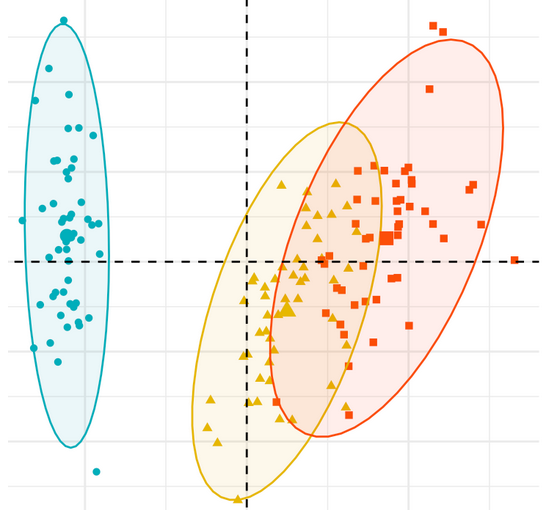
\includegraphics[height=8cm]{logos/accueil.png}
\end{center}
\vspace{10mm}

\textbf{Mémoire présenté et soutenu à Paris}

\textbf{En septembre 2021, par}

\Large {\color{Prune} \textbf{Kim ANTUNEZ}}

\vspace{15mm}

\flushleft \normalsize \textbf{Composition du jury~:}
\bigskip

\scriptsize
\arrayrulecolor{Prune}
\begin{tabular}{|p{4cm}l}
\textbf{Ivaylo Petev} &  Enseignant-chercheur en sociologie (CREST, ENSAE)\\
Directeur de mémoire & \\
\textbf{Nicolas Robette} &  Enseignant-chercheur en sociologie (CREST, ENSAE)\\
 & \\
% \textbf{} &  \\
%  & \\
% \textbf{} &  \\
%  & \\
% \textbf{} &  \\
%  & \\
% \textbf{} &  \\
%  & \\
\end{tabular}
% \begin{tabular}{p{8cm}l}
% & \\
% \textbf{} &  \\
%  & \\
% \textbf{} &  \\
%  & \\
% \textbf{} &  \\
%  & \\
% \end{tabular}

\end{titlepage}
\addamargin % this add the margin back

\frontmatter % this stuff will be roman-numbered
\pagestyle{empty} % this removes page numbers from the frontmatter
  \begin{acknowledgements}
    TODO
  \end{acknowledgements}
  \begin{abstract}
    TODO
  \end{abstract}
% 
  \hypersetup{linkcolor=black}
  \setcounter{secnumdepth}{2}
  \setcounter{tocdepth}{2}
  \tableofcontents




\mainmatter % here the regular arabic numbering starts
\pagestyle{fancyplain} % turns page numbering back on

\hypertarget{introduction}{%
\chapter*{Introduction}\label{introduction}}
\addcontentsline{toc}{chapter}{Introduction}

Il existe de nombreuses façons de définir et donc de mesurer la pauvreté. On mesure tout d'abord la pauvreté monétaire, indicateur célèbre d'inégalité mesuré notamment par les revenus, le niveau de vie, le patrimoine immobilier et financier. Il y a également en France la pauvreté institutionnelle, c'est-à-dire la relation d'assistance nouée avec l'Etat (bénéficier de certaines prestations sociales). Il existe enfin une approche subjective de la pauvreté, selon laquelle les ménages indiquent par exemple se considérer pauvre (sentiment de pauvreté) ou craindre de le devenir, ressentent un besoin de davantage d'aides publiques ou indiquent disposer d'un revenu inférieur au revenu minimum nécessaire pour vivre convenablement.
\begin{figure}

{\centering 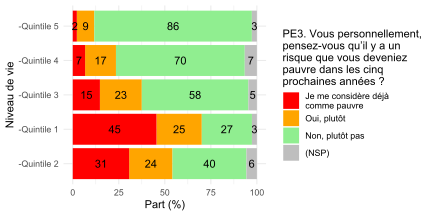
\includegraphics{M2_ANTUNEZ_SQD_files/figure-latex/figintro-1} 

}

\caption{Sentiment de pauvreté en fonction du niveau de vie en 2019}\label{fig:figintro}
\end{figure}
\begin{note}
\emph{Champ : Personnes d'au moins 18 ans résidant en France métropolitaine.}

\emph{Source : Baromètre d'opinion de la DREES, 2019.}

\end{note}
La considération de cette dimension subjective a permis à Duvoux \& Papuchon (2018) de mettre en exergue dans leur article de 2018 certains non-recoupements entre celle-ci et les dimensions objectives de la pauvreté traditionnellement analysées (monétaire et institutionnelle). En effet, certaines populations, bien que non pauvres monétairement, s'estiment pauvres. C'est notamment le cas de 2 \% des personnes appartenant à des ménages du dernier quintile de niveau de vie en 2019 (figure \ref{fig:figintro}, Baromètre d'opinion de la Drees). A l'inverse, certaines personnes bien qu'objectivement pauvres, ne se déclarent pas comme telles (plus de la moitié des personnes appartenant au premier quintile de niveau de vie). On parle alors d'un « halo » de la pauvreté qui illustre la difficulté, du fait de la complexité du phénomène de pauvreté, de capter uniquement par des mesures statistiques traditionnelles les personnes pauvres ou celles risquant de le devenir. Ce halo peut être approché par un certain nombre d'indicateurs de précarité, présents dans les bases de données, c'est-à-dire des facteurs de risques, comme la pauvreté institutionnelle, étant susceptibles de faire basculer certaines populations dans la pauvreté ou de la rendre durable comme la situation par rapport au marché du travail (contrat précaire, temps partiel, chômage\ldots), le statut d'occupation du logement (locataire, logé gratuitement\ldots), ou encore certaines configurations familiales (vivre seul, familles monoparentales\ldots).

La pauvreté subjective est un autre moyen, proposé par Duvoux \& Papuchon (2018), de réfléchir aux contours de ce halo de la pauvreté. Elle peut en effet permettre de donner des informations implicites complémentaires aux mesures institutionnelle et monétaire de la pauvreté : par exemple sur les expériences antérieures de précarité des individus, ou sur la crainte de devoir (à nouveau) y faire face (insécurité sociale), en lien également avec le contexte socio-économique dans lequel ils vivent (période de crise\ldots).

Dans ce mémoire de Master 2, nous chercherons à objectiver empiriquement les contours du halo grâce aux dimensions monétaire, institutionnelle et subjective de la pauvreté, identifiées dans la littérature. Nous modéliserons statistiquement les interactions entre ces différentes dimensions, en mettant en exergue des caractéristiques de la pauvreté non observées lorsque que ces dimensions sont étudiées individuellement. Quelles sont ces interactions, comment sont-elles situées socialement, que nous disent-elles sur l'étendue et la nature du phénomène de pauvreté ?
Pour répondre à ces questions, nous mobiliserons les données du Baromètre d'opinion de la Drees, comme Duvoux \& Papuchon (2018). Cette enquête suit chaque année depuis 2000 l'évolution de la perception des inégalités sociales et du système de protection sociale en France. Elle permet de mesurer la plupart des dimensions de la pauvreté évoquées plus haut, objectives comme subjectives.

Dans un premier temps, les méthodes économétriques classiques que nous mobiliserons nous permettront de déceler les variables permettant le plus d'expliquer la pauvreté subjective et en particulier le sentiment de pauvreté. Puis, dans un second temps, nous pousserons notre analyse un peu plus loin en cherchant à modéliser l'espace social de la pauvreté grâce à une analyse en classes latentes. Cette vision synthétique de la pauvreté devrait permettre de prolonger les travaux de Duvoux \& Papuchon (2018) en situant et quantifiant le rôle de chacune des dimensions de la pauvreté, en particulier la pauvreté subjective. L'identification du rôle joué par les différents facteurs de la pauvreté et des populations principalement concernées est en effet utile pour décrypter les leviers sur lesquels agir pour lutter contre la pauvreté et l'exclusion sociale.

\hypertarget{chap1}{%
\chapter{Dimensions de la pauvreté : perspectives théoriques}\label{chap1}}

S'il est désormais largement reconnu que la pauvreté est multidimensionnelle, l'identification de ses différentes dimensions et de la manière dont elles interagissent ne fait pas consensus. Dans cette revue de littérature\footnote{Cette revue de littérature a été guidée et facilitée par l'excellent article de blog de Auzuret (2020)}, nous présenterons tout d'abord les différentes théories et mesures de la pauvreté (partie \ref{sec:multidim}). Puis, dans la partie \ref{sec:pauvsubj}, nous décrirons plus précisément l'approche subjective de la pauvreté, développée en particulier dans le cas de la France dans Duvoux \& Papuchon (2018). Enfin, ces différents éléments nous amèneront à exposer la démarche de ce mémoire en partie \ref{sec:objmem} visant à l'étude de l'interaction entre les dimensions de la pauvreté présentes dans le Baromètre d'opinion de la Drees, base de données que nous mobilisons.

\hypertarget{sec:multidim}{%
\section{La multidimensionnalité de la pauvreté soulignée dans la littérature}\label{sec:multidim}}

\hypertarget{sec:monetaire}{%
\subsection{Pauvreté monétaire}\label{sec:monetaire}}

Puisque nous vivons dans des sociétés marchandes, dans lesquelles tout bien ou service est mesuré monétairement, la question de la pauvreté est directement liée à la notion de revenus. La pauvreté est donc en premier lieu monétaire et se mesure en général au niveau du ménage, si l'on valide l'hypothèse fondamentale de mise en commun des ressources. Le repérage des ménages pauvres résulte de la comparaison de leur niveau de vie (leur revenu disponible rapporté au nombre d'unités de consommation du ménage) avec un seuil de pauvreté. Ce dernier est, en France et en Union Européenne en général, déterminé de manière relative (en général 50 ou 60 \% du revenu médian par UC des ménages). En 2018, en France métropolitaine, le seuil de pauvreté s'établissait pour une personne seule à 1\,063 euros par mois (Demaison, Grivet, Lesdos, \& Maury-Duprey (2020)).

Une première critique adressée à l'indicateur du seuil de pauvreté est qu'une grande partie du revenu est utilisé pour des dépenses dites « pré-engagées ». C'est d'ailleurs ce que le mouvement des « Gilets Jaunes » a permis de mettre en exergue en France durant l'hiver 2018 : même avec un emploi et des revenus relativement stables, un certain nombre de ménages ne parvenaient pas à boucler leurs fins de mois en raison de ces dépenses incompressibles, le tout dans un contexte de précarité montante (emplois à temps partiel, stagnation des salaires, inflation, en particulier des loyers, etc.). Outre les « besoins primaires » (Rawls (2020)) liés à la santé et à l'autonomie (se nourrir, se loger\ldots), doit-on prendre en considération d'autres (voire tous) éléments du mode de vie pour étudier le phénomène de la pauvreté ? C'est notamment ce que pense l'économiste et philosophe indien Amartya Sen.~Dans Sen (1985), il met l'accent sur la notion de « capacité », c'est-à-dire la liberté que doit avoir un individu de choisir entre différentes vies possibles, des souhaits qui varient selon les individus, et à un niveau plus large, selon les sociétés. Une étude de la Drees (Lelièvre \& Rémila (2018)) propose une mesure du seuil de pauvreté en déduisant des revenus les dépenses pré-engagées, et montre que les inégalités de niveau de vie sont encore plus marquées une fois qu'elles sont prises en compte.

Par ailleurs, la mesure relative de la pauvreté monétaire ne permet pas d'appréhender les différences de situations qui peuvent correspondre à un même niveau de vie et rend également difficile les comparaisons internationales. C'est pourquoi certaines méthodologies sont proposées afin d'étudier la pauvreté monétaire absolue -- également appelée privation matérielle -- qui correspond à un niveau de vie inférieur à la valeur d'un « panier » de biens et services dont la disposition est jugée nécessaire pour satisfaire certains besoins considérés comme essentiels. Dans l'Union européenne, une personne est réputée en situation de privation matérielle et sociale si elle déclare ne pas avoir les ressources financières suffisantes pour couvrir les dépenses liées à au moins cinq éléments de la vie courante sur treize considérés comme très souhaitables pour avoir un niveau de vie acceptable\footnote{Le dispositif européen EU‑SILC sur les revenus et les conditions de vie (Eurostat) permet d'apprécier les différences et les points communs entre pauvreté monétaire et privation matérielle et sociale.}.

Dans la même logique, l'Observatoire national de la pauvreté (Onpes) a publié des budgets de référence établis grâce à une concertation mêlant citoyens et experts. Pour chaque type de ménage (actif isolé, retraité isolé, couple d'actifs sans enfants, etc.), une liste précise de biens et de services jugés nécessaires pour participer effectivement à la vie sociale a été établie. Le montant des budgets minima de référence sont situés entre 1 424 euros et 3 284 euros, selon le type de ménage (ONPES (2015)).

\hypertarget{sec:institutionnelle}{%
\subsection{Pauvreté instititionnelle}\label{sec:institutionnelle}}

Outre la conception monétaire de la pauvreté, l'approche institutionnelle de la pauvreté compte le nombre de ménages pauvres à partir de ceux bénéficiant des minima sociaux, c'est-à-dire d'un revenu minimum garanti basé sur des critères établis par l'État. En 2018, 11 \% de la population française était couverte par les minima sociaux, si l'on compte les conjoints et enfants à charge des bénéficiaires (Calvo (2019)).

Cette approche est inspirée de Georg Simmel et s'est développée dans un contexte du développement du chômage de masse à la suite duquel la pauvreté est devenue un objet d'intervention publique. La pauvreté institutionnelle renseigne alors sur la relation d'assistance qui lie l'individu à la société (Simmel (1998)). Selon Simmel, c'est la société qui définit en partie la pauvreté par les normes auxquelles elle se réfère pour venir en aide aux populations. Cette relation d'assistance définit la pauvreté comme une identité (Paugam \& Schnapper (1991)), plus encore qu'un état d'une personne manquant de biens matériels. Elle correspond à un statut social spécifique et dévalorisé, comme l'illustre très bien l'expression « cas sociaux » faisant référence à la fois à une situation entraînant des risques d'exclusion sociale nécessitant une prise en charge par la société mais aussi à un groupe social d'individus étant dans cette condition.
Or, cette relation d'assistance qui se noue avec l'Etat diffère fortement selon les cultures et les pays. Dans Esping-Andersen (1990), l'auteur décrit les processus d'émergence des trois types de régimes sociaux en Europe. Cette typologie a contribué à la considération de la protection sociale comme une dimension déterminante dans la compréhension des structures sociales des sociétés contemporaines, en lien notamment avec les politiques de luttes contre les inégalités sociales et la pauvreté. Tout d'abord, le modèle social-démocrate, le plus universaliste, accorde les mêmes droits à l'ensemble des citoyens. Le modèle libéral se fonde sur une sécurité plus minimale destinée aux personnes les plus dans le besoin. Enfin, le modèle bismarckien, auquel la France est souvent rattachée tout comme l'Allemagne, vise à maintenir un revenu en dépit des risques sociaux grâce à une assurance sociale obligatoire. Le Baromètre d'opinion de la Drees permet de voir qu'en dépit de la dominante bismarckienne du système de sécurité sociale français, les Français sont particulièrement attachés à l'universalité de certaines prestations sociales (Grislain-Letrémy \& Papuchon (2017)).

L'étude de la pauvreté ne peut donc pas se faire sans analyser en parallèle le rôle des pouvoirs publics dans la lutte contre la pauvreté. Ils peuvent en effet impulser des mesures pour augmenter les ressources des ménages (prestations sociales, baisses d'impôts\ldots) comme en France lors de la récente « Loi portant mesures d'urgence économiques et sociales » adoptée fin décembre 2018 à la suite du mouvement des « Gilets Jaunes » qui a amené notamment à revaloriser la prime d'activité. Plus anciennement, le « plan pluriannuel contre la pauvreté et pour l'inclusion sociale » de 2013 visait, en plus de réduire les inégalités, à davantage accompagner les citoyens vers l'insertion. Enfin, les pouvoirs publics insistent également beaucoup sur des politiques de reprise de l'emploi (comme le développement de l'apprentissage\footnote{Dans Cahuc, Ferracci, Tirole, \& Wasmer (2014), les auteurs montrent que, contrairement à d'autres pays, l'expansion des effectifs d'apprentis a essentiellement bénéficié aux jeunes déjà diplômés en France. Les auteurs l'expliquent par la complexité du circuit de formation professionnelle en alternance français, par la perception trop peu positive de cette orientation par le corps enseignant ou encore par la non-adéquation des formations d'apprentissage avec les besoins des entreprises.}) comme moyen de faire baisser le niveau de pauvreté. Toutefois, l'existence d'emplois de plus en plus précaires invitent à complexifier l'analyse purement monétaire de la pauvreté décrite en partie \ref{sec:monetaire}.

\hypertarget{le-halo-de-la-pauvretuxe9}{%
\subsection{Le halo de la pauvreté}\label{le-halo-de-la-pauvretuxe9}}

Les différentes dimensions et mesures de la pauvreté font souvent l'objet d'analyses sociologiques indépendantes, bien qu'elles interagissant en réalité les unes avec les autres. Le brouillage des frontières entre les différentes causes potentielles de la pauvreté est appelé « halo de la pauvreté ». Ces causes sont appelées ici « facteurs de précarité », faisant référence, comme dans CINGOLANI (2005) à des facteurs de risques étant susceptibles de faire basculer certaines populations plus que d'autres dans la pauvreté : temps partiels, CDD, travail intérimaire, chômage, accidents de la vie divers\ldots{}

Certaines franges de la population ont ainsi une position sociale durablement jugée inférieure sur une échelle de prestige ainsi que des difficultés à se projeter dans l'avenir : cela peut être dû à leur situation familiale (monoparentalité, famille nombreuse\ldots) ou encore aux déséquilibres du marché de l'emploi évoqué ci-dessus qui amènent à l'existence de « travailleurs pauvres » (Ponthieux (2004)). Par ailleurs, un même niveau de pauvreté n'a pas la même signification selon s'il correspond à une situation durable (ancrage dans la pauvreté) ou plus ponctuelle, c'est pourquoi il est également important d'étudier des indicateurs de dynamiques de pauvreté en plus des indicateurs d'état. Cela peut être rendu possible grâce à des analyses longitudinales de la pauvreté comme celle de Lollivier \& Verger (2005), mais celles-ci demeurent rares car les données quantitatives sont elles-mêmes rares.

\hypertarget{sec:pauvsubj}{%
\section{L'apport de la dimension subjective dans l'étude de la pauvreté}\label{sec:pauvsubj}}

\hypertarget{pauvretuxe9-subjective}{%
\subsection{Pauvreté subjective}\label{pauvretuxe9-subjective}}

L'approche subjective de la pauvreté s'appuie sur la manière dont les individus perçoivent leur situation. Il existe deux approches principales dans la littérature française et internationale.

La première s'intéresse aux difficultés financières perçues en mettant notamment en relation le niveau de vie minimum nécessaire tel qu'il ressort d'enquêtes auprès d'individus au niveau de vie dont ils disposent effectivement. Cette approche permet d'élaborer des seuils de pauvreté subjective (\emph{subjective poverty lines}, Veit-Wilson (1987)) et d'effectuer des comparaisons internationales sur le sujet (Paugam (2002) ; Paugam \& Selz (2005)) mais ne permet probablement pas réellement aux individus de s'affranchir des normes sociales quand ils formulent leurs réponses (Spicker, Franzoni, Leguizamón, \& Gordon (2007), p.~199).

La seconde s'intéresse à des indicateurs de privation (\emph{deprivation indicator approach}, Mack, Lansley, \& others (1985)) telle que la mesure de la pauvreté monétaire absolue présentée plus haut qui s'intéresse à l'accès à un panier de biens et services jugés essentiels par la population.

Ces deux approches subjectives se fondent toutefois principalement sur une approche monétaire de la pauvreté qui est donc qualifiable « d'indirecte ». C'est la raison pour laquelle d'autres mesures s'intéressent également à des mesures plus « directes » de la pauvreté subjective en demandant, aux individus de s'auto-classer au niveau de la hiérarchie sociale, mais utiliser ce résultat comme mesure subjective de la pauvreté suppose les notions de pauvreté et d'intégration sociale sont assimilables, et met de côté le lien avec l'insécurité sociale.

\hypertarget{sec:approcheduvoux}{%
\subsection{L'approche de Duvoux et Papuchon}\label{sec:approcheduvoux}}

Les travaux de Duvoux \& Papuchon (2018) confrontent les mesures monétaires et institutionnelles de la pauvreté à plusieurs mesures subjectives collectées dans le Baromètre d'opinion de la Drees. De cette manière, la pauvreté est définie de manière inductive par son aspect subjective sans pour autant mettre de côté l'objectivation permise par les indicateurs classiques de statistique publique.

La principale mesure correspond au sentiment de pauvreté, une indicatrice des individus qui déclarent se sentir pauvre\footnote{ Cette mesure de la pauvreté pourrait même permettre de discuter de l'évidence (ou non) du ménage comme unité de mesure de la pauvreté.} (voir la question \texttt{PE3} en annexe \ref{annexequestio}). En 2019, c'était le cas de 19 \% des Français\footnote{ L'ensemble de ces chiffres ne concernent que les individus ayant souhaité s'exprimer (chiffres sans les « ne se prononcent pas »).}. Leur étude mobilise également, dans une moindre mesure deux autres approches de la pauvreté subjective : une qui s'intéresse au besoin d'aide publique (question \texttt{PE15}) et une autre sur les difficultés financières perçues qui mesure l'écart entre le revenu du ménage du répondant (qu'il déclare) et celui dont un foyer comme le sien doit selon lui disposer au minimum pour vivre (question \texttt{PE16}).

Ces différentes mesures de pauvreté subjective leur permettent de montrer que les mesures traditionnelles (monétaire et institutionnelles) de la pauvreté sont trop réductrices. En particulier, l'approche relationnelle d'assistance de Simmel rétrécit selon les auteurs le périmètre de la pauvreté puisque certains publics ne sont pas pris en charge par les aides sociales et que par ailleurs, le non-recours au prestations sociales est un sujet particulièrement présent en France. Ils cherchent donc à valider empiriquement le recours au sentiment de pauvreté en complément des indicateurs traditionnels.

En mettant en lumières le non-recoupement des définitions, ils cherchent à toucher du doigt le halo de la pauvreté évoqué plus haut. Certaines populations, bien que non pauvres monétairement, s'estiment pauvres. C'est notamment le cas de respectivement 2 \% et 7 \% des personnes appartenant à des ménages du quatrième et dernier quintile de niveau de vie en 2019 (figure \ref{fig:figintro}). A l'inverse, certaines personnes bien qu'objectivement pauvres, ne se déclarent pas comme telles (plus de la moitié des personnes appartenant au premier quintile de niveau de vie). Ils apportent une illustration à la thèse selon laquelle le sentiment de pauvreté ne concerne pas que les personnes en situation d'assistance ou éloignées du marché du travail mais concerne également une partie des personnes en emploi, notamment les ouvriers et les employés.

Enfin, ils insistent sur l'appréciation négative portée par les personnes qui se déclarent pauvres sur leur trajectoire passée et leur avenir et en concluent que « la pauvreté subjective se comprend sociologiquement comme un indicateur d'insécurité sociale durable ». Ce point précis a fait l'objet de quelques controverses sociologiques exposées dans la partie \ref{sec:limitesduvoux} qui suit.

\hypertarget{sec:limitesduvoux}{%
\subsection{Les limites identifiées d'une telle approche}\label{sec:limitesduvoux}}

Cet article a été l'origine de deux discussions (Paugam (2020) et Lahieyte (2020)) permettant de revenir sur l'approche proposée par les précédents auteurs.

Les débats portent tout d'abord sur des inquiétudes concernant d'éventuels biais de la mesure du sentiment de pauvreté. Comme dans toute enquête, d'autant plus s'agissant d'une enquête d'opinion, les réponses sont liées à la formulation de la question. Or, cette question semble imprécise selon plusieurs aspects, ce qui rend difficile l'identification de ce qui est réellement mesuré : on ne sait pas ce que les enquêtés entendent par « un foyer comme le leur » et font-ils bien dans leurs réponses référence au revenu de leur ménage ou bien uniquement au leur ? Les réponses dépendent également du rapport qui se tisse entre enquêteur et enquêté : il est fort probable que certaines personnes pourraient ne pas oser se déclarer comme pauvre. D'ailleurs, le fort pourcentage de non-réponse à cette question (6 \% en 2019 contre un maximum de 1 ou 2 pourcents pour la plupart des questions de l'enquête) va dans le sens de cette interprétation. C'est pourquoi Duvoux \& Papuchon (2020) recommandent de s'intéresser davantage à l'interprétation des résultats en gardant en tête le fait que cet indicateur est un proxy permettant de mesurer tout un ensemble d'éléments complexes à appréhender, comme dans toute enquête d'opinion.

D'après Paugam (2020), les auteurs opposent également trop souvent l'aspect subjectif (pauvreté déclarée) à l'aspect institutionnel (perception de minima sociaux) et devraient davantage faire le lien entre les deux. Selon Paugam, le sentiment d'être pauvre serait prioritairement mise en lien par les auteurs avec le climat d'insécurité sociale qui accompagne la crise salariale et pas assez à la prise en charge institutionnelle de l'assistance montrée par Simmel. Pourtant, toujours selon Paugam, le développement de l'assistance est depuis les années 1980, en France et dans les pays occidentaux, une conséquence directe de la précarisation des emplois et de la montée du chômage.

De manière générale, Duvoux et Papuchon partent de l'hypothèse que leur mesure du sentiment de pauvreté traduit avant tout une condition d'insécurité sociale, c'est-à-dire de déficit de garantie face à l'avenir. Or, ils oublient selon Paugam une autre interprétation plus importante : l'infériorité sociale, c'est-à-dire le manque de reconnaissance sociale et le sentiment d'inutilité sociale. Ces différents éléments d'explication peuvent d'ailleurs être en partie testées grâce aux données des modules « opinion générale » et « pauvreté / exclusion » du Baromètre de la Drees. Concernant l'insécurité sociale, on interroge notamment les Français sur leur optimisme face à l'avenir (pour eux, mais aussi pour les générations futures) et sur leur vision sur l'évolution passée et à venir des inégalités d'une part et de la pauvreté et l'exclusion d'autre part. Pour l'infériorité sociale, l'appréciation des Français sur la manière (de très mauvaise à très bonne) dont ils considèrent leur situation actuelle ou sur leur sentiment ou non d'avoir une situation que leur parent au même âge (déclassement intergénérationnel) permettra d'éclairer également une partie du phénomène.

\hypertarget{sec:objmem}{%
\section{Etudier les interactions entre les dimensions de la pauvreté}\label{sec:objmem}}

La pauvreté, en plus d'être multidimensionnelle et de reposer sur des dimensions qui ne se recoupent pas entièrement, dépend donc aussi de situations individuelles particulières et de facteurs potentiellement inobservables. Cela explique la difficulté méthodologique de définir ce phénomène. Quand bien même on arriverait à définir les indicateurs les plus pertinents, il faudrait ensuite définir un moyen de construire une échelle de la pauvreté. Or, dès lors que l'on sort du cadre de l'unidimensionnalité, on ne dispose pas d'une méthode correcte pour classer sans ambiguïté les individus. Et peut-on vraiment considérer la pauvreté comme étant ordinale quand on se base sur les théories de liberté de choix individuels et de pluralisme des goûts comme le fait Sen (1985) ?

Cette complexité du sujet même de pauvreté et les débats sur la détermination de ses dimensions a fait naître des initiatives internationales de recherche participative sur les dimensions de la pauvreté comme celle de l'association Monde (2019). Des personnes en situation de pauvreté, des professionnels et des universitaires de différents pays\footnote{Au Bangladesh, en Bolivie, en France, en Tanzanie, au Royaume-Uni et aux États-Unis.} ont travaillé ensemble pour aboutir à trois groupes de dimensions de la pauvreté (figure \ref{fig:figatd}) interdépendantes faisant la synthèse de ce qui a été évoqué précédemment. Le premier groupe, situé au centre de la figure \ref{fig:figatd}, forme le cœur de l'expérience de la pauvreté : les souffrances physiques ou mentales résultant de la dépossession du pouvoir d'agir (le manque de contrôle sur sa vie), causées par les privations auxquelles les personnes réagissent par de la lutte et de la résistance. Un deuxième groupe rassemble les dimensions relationnelles de la pauvreté : les maltraitances institutionnelles (incapacité des institutions à répondre aux besoins), sociales (par d'autres groupes sociaux) et les compétences non reconnues des personnes en situation de pauvreté. Le dernier groupe rassemble les privations : le manque de travail décent, le revenu insuffisant et les privations matérielles et sociales. Les neuf dimensions évoquées, et donc l'intensité de la pauvreté, peuvent être modifiées par cinq facteurs : l'identité (genre, appartenance ethnique, etc.), le temps (le moment de la vie où elle est vécue), le lieu (pays mais aussi urbain versus rural), l'environnement (météo, inondations, sècheresse\ldots) ainsi que les croyances culturelles : la société en elle-même impulse des dépenses obligatoires dans le cadre de traditions qui jouent sur les revenus (la dot, les cadeaux\ldots).
\begin{figure}

{\centering 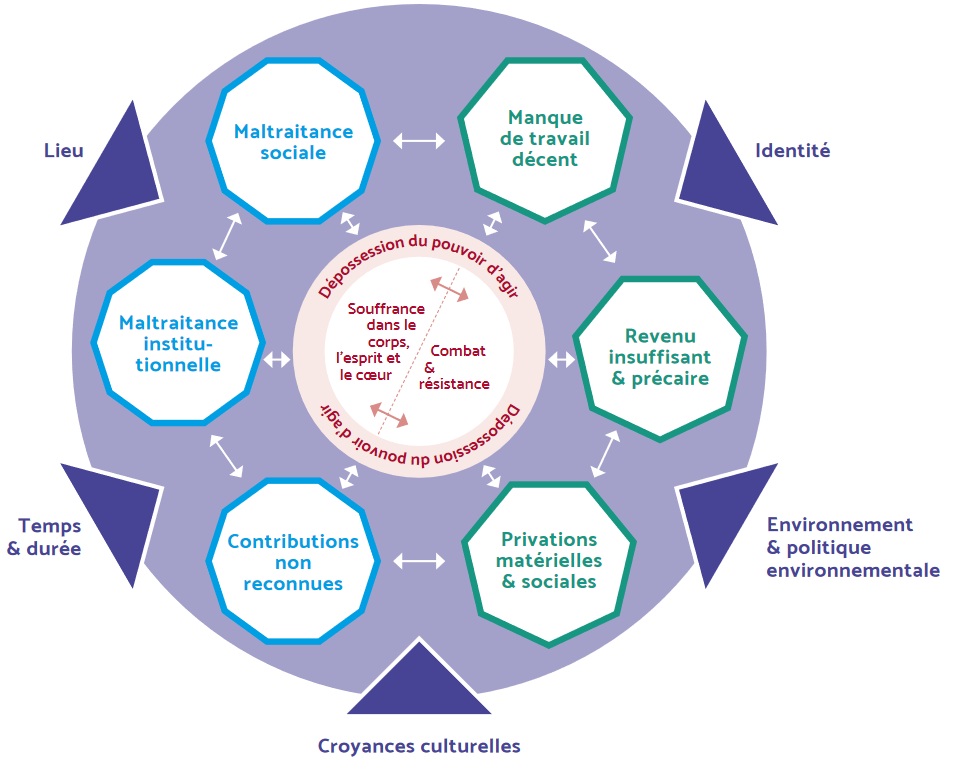
\includegraphics[width=0.8\linewidth]{figures/fig_atd} 

}

\caption{Graphique sur les dimensions de la pauvreté}\label{fig:figatd}
\end{figure}
\begin{note}
\emph{Source : ATD Quart Monde et Université d'Oxford, janvier 2019}

\end{note}
Dans le cadre de ce mémoire de Master 2, nous avons donc cherché à reconstruire empiriquement l'espace social de la pauvreté en mobilisant les différentes dimensions identifiées dans la littérature présentée dans ce chapitre \ref{chap1}. Pour cela, nous mobiliserons les données du Baromètre d'opinion de la Drees, comme Duvoux et Papuchon 2018, afin de faire intervenir la dimension subjective de la pauvreté. Nous tenterons de répondre à cet objectif grâce à des méthodes économétriques robustes, faisant notamment intervenir des analyses en classes latentes. Cette modélisation synthétique du phénomène de pauvreté devrait permettre de prolonger les travaux de Duvoux et Papuchon en situant socialement le rôle de chacune des dimensions de la pauvreté, en particulier la pauvreté subjective.

\hypertarget{probluxe9matique}{%
\subsection{Problématique}\label{probluxe9matique}}
\begin{encadre}
\textbf{A REDIGER ULTERIEUREMENT}

\end{encadre}
Le sentiment de pauvreté, mesuré de manière subjective auprès des enquêtés, est également un moyen d'identifier des composantes sous-jacentes de la pauvreté : des expériences antérieures de précarité, ou la crainte de pouvoir y (re)tomber ainsi que d'autres éléments de contextes sur le parcours spécifique de chaque individu, ainsi que sur le contexte socio-économique plus général de la société et de l'époque dans lesquelles ils vivent (période de crise\ldots).

\hypertarget{base-de-donnuxe9es-le-baromuxe8tre-dopinion-de-la-drees}{%
\subsection{Base de données : Le Baromètre d'opinion de la Drees}\label{base-de-donnuxe9es-le-baromuxe8tre-dopinion-de-la-drees}}

\hypertarget{un-outil-de-suivi-conjoncturel-depuis-2000}{%
\subsubsection{Un outil de suivi conjoncturel depuis 2000}\label{un-outil-de-suivi-conjoncturel-depuis-2000}}

Le Baromètre d'opinion de la DREES\footnote{La présentation du Baromètre faite ici est très fortement inspirée de celle proposée par la Drees dans ses publications.} recense chaque année depuis 2000 l'évolution de l'opinion des Français sur leur santé, sur la protection sociale dans l'ensemble de ses dimensions (assurance maladie, retraite, famille, handicap, dépendance, solidarité, lutte contre la pauvreté et l'exclusion) ainsi que sur les inégalités et la cohésion sociale (depuis 2014).

À la demande de la Drees, l'institut BVA réalise cette enquête en face-à-face auprès d'un échantillon de 3 000 personnes différentes chaque année, représentatif de la population habitant en France métropolitaine âgée de 18 ans et plus. Cet échantillon est construit selon la méthode des quotas, par sexe, âge, profession de la personne de référence, après stratification par région et catégorie d'agglomération.

Le caractère annuel et l'ancienneté de ce baromètre en font un outil de suivi conjoncturel de référence et indispensable pour appréhender l'évolution de l'opinion des Français sur les politiques dont le ministère des Solidarités et de la Santé a la charge, tant en matière de santé que de solidarité. Le Baromètre apporte un éclairage complémentaire aux travaux menés habituellement par la Drees, puisqu'il permet de mettre en parallèle les évolutions perçues et réelles des politiques sanitaires et sociales. Il est notamment utilisé à ce titre par des chercheurs en sociologie et en science politique.

\hypertarget{appruxe9hender-lopinion-sur-dix-thuxe9matiques}{%
\subsubsection{Appréhender l'opinion sur dix thématiques}\label{appruxe9hender-lopinion-sur-dix-thuxe9matiques}}

Le questionnaire vise à connaître les attentes et les préoccupations des Français sur le fonctionnement du système actuel et sur de potentielles réformes. Il s'articule autour de plusieurs modules thématiques cités ci-dessous. Les thèmes suivis d'un astérisque (*) sont davantage approfondis en années paires, grâce à la présence de questions supplémentaires bisannuelles. A l'inverse, les thèmes non suivis d'un astérisque sont approfondis en années impaires.
\begin{itemize}
\tightlist
\item
  Inégalités* (inégalités de revenus, inégalités entre femmes et hommes, justice sociale, etc.) ;
\item
  Pauvreté et exclusion* (évolution de la pauvreté, définition des personnes exclues, opinion sur le montant et l'efficacité du RSA et des allocations chômage, etc.) ;
\item
  Protection sociale (financement de la protection sociale, ciblage des prestations sur les plus modestes ou les seuls cotisants, etc.) ;
\item
  Retraites (âge de départ anticipé et souhaité, niveau de vie des retraités, réformes souhaitées pour préserver le système de retraite, etc.) ;
\item
  Santé (perception de l'état de santé de la population, qualité et accès aux soins, risque sanitaire, inégalités de santé, réformes souhaitées, etc.) ;
\item
  Famille* (objectif que doit poursuivre la politique familiale, durée du congé maternité, mode de garde privilégié pour les enfants en bas âge, etc.) ;
\item
  Handicap (effort de la société envers les personnes handicapées, etc.) ;
\item
  Dépendance (création d'une cotisation obligatoire pour aider financièrement les personnes dépendantes, statut des aidants, etc.) ;
\item
  Logement (difficulté pour se loger, etc.) ;
\item
  Cohésion sociale* (sentiment d'intégration, laïcité, discriminations, non-recours, etc.).
\end{itemize}
\hypertarget{pruxe9cautions-dinterpruxe9tation-des-enquuxeates-dopinion}{%
\subsubsection{Précautions d'interprétation des enquêtes d'opinion}\label{pruxe9cautions-dinterpruxe9tation-des-enquuxeates-dopinion}}

Les réponses à une enquête d'opinion sont particulièrement sensibles à la formulation des questions et à leur place dans le questionnaire. Du fait de l'ancienneté et de la stabilité du questionnaire du Baromètre, ses différentes éditions permettent néanmoins des comparaisons entre catégories (selon le revenu, l'âge, etc.) et dans le temps. Toutefois, compte tenu de la taille de l'échantillon, de faibles variations peuvent ne refléter que des imperfections de mesure. Par souci de simplification, les résultats présentés sont calculés en excluant les réponses « ne se prononce pas » (NSP). Lorsque celles-ci dépassent 3 \% des réponses, une annotation spécifique est ajoutée à la figure concernée ou en note dans le texte.

\hypertarget{accuxe9der-aux-donnuxe9es}{%
\subsubsection{Accéder aux données}\label{accuxe9der-aux-donnuxe9es}}

Les bases contenant l'intégralité des données individuelles du Baromètre d'opinion de la Drees sont en libre accès depuis 2019. Elles sont mises en ligne sur leur \href{http://www.data.drees.sante.gouv.fr/}{plateforme de diffusion de données} . Elles sont accompagnées de fichiers Excel présentant les résultats pour chaque question en historique (tris à plat) et les résultats croisés avec les principales variables sociodémographiques pour la dernière année disponible (tris croisés). Un \href{http://dataviz.drees.solidarites-sante.gouv.fr/Barometre-DREES}{outil de visualisation interactive} permet de visualiser et télécharger sous forme de tableaux et graphiques l'ensemble des résultats du Baromètre d'opinion de la DREES depuis 2000. Plus d'informations sont disponibles sur la \href{https://drees.solidarites-sante.gouv.fr/etudes-et-statistiques/open-data/aide-et-action-sociale/article/le-barometre-d-opinion-de-la-drees}{page internet de la DREES dédiée au Baromètre}.

\hypertarget{sec:methodo}{%
\subsection{Méthodologie}\label{sec:methodo}}

\hypertarget{sec:mesures}{%
\subsubsection{Stratégie empirique et mesures}\label{sec:mesures}}

Dans cette étude, nous compilons les réponses obtenues lors des quatre dernières vagues d'enquêtes (2016, 2017, 2018 et 2019) pour avoir des effectifs suffisants (plus de 12 000 répondants) ceci afin d'obtenir des résultats significatifs, sans pour autant mobiliser des données trop anciennes. Les données ont été collectées avant la crise sanitaire du Covid-19, ce qui permet de ne pas faire intervenir un certain nombre de facteurs d'incertitudes liés à cette crise dans notre analyse. Il est à noter que le Baromètre \textbf{n'est pas un panel} et que sont interrogées chaque année des personnes différentes.

Les variables de l'enquête plus particulièrement mobilisées pour cette étude sont décrites ci-dessous. Elles ont permis d'opérationnaliser les différentes dimensions de la pauvreté : monétaire, institutionnelle, et subjective, ainsi que différentes variables de contrôles, parfois facteurs de précarité. Les codes des questions font référence à ceux tels qu'ils sont référencés dans le questionnaire du Baromètre dont un extrait est reproduit en annexe \ref{annexequestio}.

Dans le Baromètre d'opinion, les enquêtés sont interrogés dans une première question sur le revenu mensuel net du ménage avant impôt tenant compte de tous les types de revenus perçus par le ménage listés auparavant dans le questionnaire\footnote{ Salaires, traitements et primes/Revenus d'une activité professionnelle indépendante/RSA (Revenu de solidarité active)/Allocations de chômage/Préretraite,
  retraites/Revenus d'actifs financiers/Revenus de locations/Prestations familiales (allocations familiales, complément familial, prestation d'accueil du jeune enfant {[}PAJE{]}\ldots)/Allocations de logement (APL,\ldots)/Prestations liées au handicap, à l'invalidité ou à la dépendance (AAH, APA, PCH\ldots)/Bourses d'études/Pensions alimentaires ou argent reçu tous les mois de la part de proches (familles, amis\ldots)}. Puis s'ils ne répondent pas à cette question, on leur propose de renseigner une tranche de revenu afin de réduire au maximum la non-réponse. Malgré ces précaution, la question des revenus reste la question avec le plus fort taux de non-réponse (X \% sur 2016 à 2019 sur le revenu en tranches et X \% sur le montant précis). Nous imputons donc le montant précis en attribuant au ménage ayant uniquement répondu à la partie en tranche la moyenne déclarée dans la variable « montants » pour les enquêtés se situant dans la même tranche (imputation par les moyennes conditionnelles). Puis, calcul du niveau de vie\footnote{ Le niveau de vie se mesure au niveau du ménage. Il est égal au revenu disponible du ménage divisé par le nombre d'unités de consommation (UC). Les unités de consommation sont généralement calculées selon l'échelle d'équivalence dite de l'OCDE modifiée qui attribue 1 UC au premier adulte du ménage, 0,5 UC aux autres personnes de 14 ans ou plus et 0,3 UC aux enfants de moins de 14 ans.}.

\hypertarget{sec:methodes}{%
\subsubsection{Méthodes statistiques utilisées}\label{sec:methodes}}

\hypertarget{la-pauvretuxe9-comme-espace-social}{%
\chapter{La pauvreté comme Espace social}\label{la-pauvretuxe9-comme-espace-social}}

\hypertarget{sec:nonreducnv}{%
\section{Le sentiment de pauvreté ne se réduit pas au niveau de vie}\label{sec:nonreducnv}}

\hypertarget{a-partir-de-2018-le-sentiment-de-pauvretuxe9-augmente-mais-ses-facteurs-explicatifs-ne-sont-pas-radicalement-modifiuxe9s}{%
\subsection{A partir de 2018, le sentiment de pauvreté augmente mais ses facteurs explicatifs ne sont pas radicalement modifiés}\label{a-partir-de-2018-le-sentiment-de-pauvretuxe9-augmente-mais-ses-facteurs-explicatifs-ne-sont-pas-radicalement-modifiuxe9s}}

Le Baromètre d'opinion de la Drees permet de mesurer le niveau et l'évolution au cours du temps du sentiment de pauvreté\footnote{Pour rappel, le sentiment de pauvreté s'appréhende dans le Baromètre d'opinion par la proportion de Français qui, à la question \texttt{PE3} « Et vous personnellement, pensez-vous qu'il y a un risque que vous deveniez pauvre dans les cinq prochaines années ? », répondent « Je me considère déjà comme pauvre » (voir extrait de questionnaire en annexe \ref{annexequestio}).} des Français. Les données de l'enquête permettent d'observer que le sentiment de pauvreté a sensiblement augmenté ces dernières années, en particulier depuis 2018, pour atteindre 19 \% en 2019 (figure \ref{fig:figchap1compa20152019}). Il en va de même pour les difficultés financières perçues, à savoir la mise en relation du niveau de vie minimum nécessaire pour vivre selon les enquêtés au niveau de vie dont ils disposent effectivement\footnote{quand la réponse à la question \texttt{PE16} « Selon vous, pour vivre, quel est le montant dont doit disposer AU MINIMUM un foyer comme le vôtre, par mois (en euros) ? » est inférieure à celle de la question \texttt{SDREVCL} « Nous désirons savoir à quel niveau de revenus MENSUELS NETS AVANT IMPOTS se situe votre foyer » dont on a imputé de la non-réponse (voir partie \ref{sec:mesures})}, qui concernent plus de la moitié des Français, et ce depuis les cinq dernières années.
\begin{figure}

{\centering 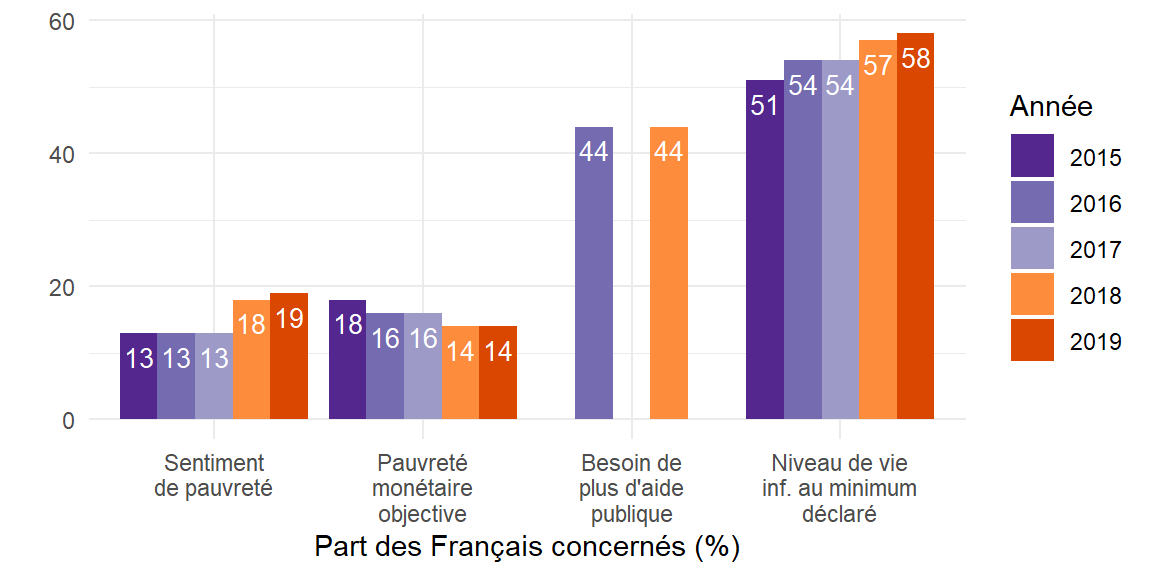
\includegraphics{M2_ANTUNEZ_SQD_files/figure-latex/figchap1compa20152019-1} 

}

\caption{Différents indicateurs de pauvreté (2015 à 2019)}\label{fig:figchap1compa20152019}
\end{figure}
\begin{note}
\emph{Champ : Personnes d'au moins 18 ans résidant en France métropolitaine.}

\emph{Source : Baromètre d'opinion de la DREES, 2015-2019.}

\end{note}
En parallèle, la pauvreté objective -- qui correspond à la proportion de Français en dessous du seuil de pauvreté (seuil de 60 \% du revenu médian\footnote{Cet indicateur ne correspond pas aux données nationales officielles mais à un calcul avec les données du Baromètre. La source qui fait référence en France pour le taux de pauvreté (Insee, ERFS) donne, elle, des taux en légère augmentation depuis 2015 : 14,3 \% pour 2015, 13,9 \% pour 2016, 14,1 \% pour 2017 et 14,8 \% pour 2018.}) diminue légèrement et atteint 14 \% en 2019. Enfin, 44 \% des Français jugent en 2019 ne pas être suffisamment aidés par les pouvoirs publics\footnote{Réponse « Vous auriez besoin d'être aidé(e) davantage par les pouvoir publics » à la question \texttt{PE15} : « Actuellement, compte tenu de votre situation globale, du montant des aides publiques (RSA, allocations familiales, aides au logement), et du montant de vos impôts, vous considérez que\ldots{} ». Cette question est posée uniquement en \textbf{années paires}.}.

Pour expliquer le sentiment de pauvreté, un premier modèle de régression logistique où le fait de se déclarer pauvre constitue la variable dépendante est utilisé. Ses résultats sont présentés en tableau \ref{tab:tabcompa}. On remarquera dans les dernières lignes de celui-ci que les années 2018 et 2019 sont très significativement positives dans le modèle appliqué sur la base compilant les années 2016 à 2019, majoritairement utilisée pour ce mémoire. Ce résultat est cohérent avec l'évolution observée en figure \ref{fig:figchap1compa20152019} commentée précédemment. Malgré la brusque augmentation du sentiment de pauvreté observée depuis 2018, les autres coefficients du modèle actualisé sont globalement semblables à ceux du modèle appliqué sur les données plus anciennes (2015---2017). En d'autres termes, cela semble signifier que, même si le sentiment de pauvreté a augmenté en niveau depuis 2018, ses déterminants n'ont pas sensiblement changé dans le temps (sauf petites exceptions décrites ci-après).
\begin{longtable}[t]{>{\raggedright\arraybackslash}p{4cm}>{\raggedright\arraybackslash}p{6cm}>{\raggedright\arraybackslash}p{2cm}>{\raggedright\arraybackslash}p{2cm}}
\caption{\label{tab:tabcompa}Réactualisation du modèle 1 de Duvoux et Papuchon (2018)}\\
\toprule
Modèle logit &  Variable dépendante : se déclarer pauvre & Odds ratio - Années 2015 à 2017 & Odds ratio - Années 2016 à 2019\\
\midrule
\endfirsthead
\caption[]{\label{tab:tabcompa}Réactualisation du modèle 1 de Duvoux et Papuchon (2018) \textit{(suite)}}\\
\toprule
Modèle logit &  Variable dépendante : se déclarer pauvre & Odds ratio - Années 2015 à 2017 & Odds ratio - Années 2016 à 2019\\
\midrule
\endhead
\midrule
\multicolumn{4}{r@{}}{\textit{(suite en page suivante...)}}\
\endfoot
\bottomrule
\multicolumn{4}{l}{\rule{0pt}{1em}\textit{Note: }}\\
\multicolumn{4}{l}{\rule{0pt}{1em}Modèle 2015-2017 : N = 8460 et \$R\textasciicircum{}2\$ ajusté = 24,8 \% / Modèle 2016-2019 : N = 10759 et \$R\textasciicircum{}2\$ ajusté = 25,9 \%.}\\
\multicolumn{4}{l}{\rule{0pt}{1em}* : significatif au seuil de 5 \% ; ** : 1 \% ; *** : 0,1 \%.}\\
\endlastfoot
Niveau de vie & Quintile 1 & 1,65*** & 1,49***\\
 & Quintile 2 & Réf. & Réf.\\
 & Quintile 3 & 0,48*** & 0,51***\\
 & Quintile 4 & 0,24*** & 0,24***\\
 & Quintile 5 & 0,18*** & 0,15***\\
\addlinespace
Types de ressources & Pas d'aide au logement & Réf. & Réf.\\
\cellcolor[HTML]{fcdcf4}{\textbf{perçues par le ménage}} & \cellcolor[HTML]{fcdcf4}{\textbf{Aide au logement reçue}} & \cellcolor[HTML]{fcdcf4}{\textbf{1,37***}} & \cellcolor[HTML]{fcdcf4}{\textbf{1,71***}}\\
(12 mois) & Pas de RSA & Réf. & Réf.\\
 & RSA reçu & 1,87*** & 1,73***\\
 & Pas d'alloc. hand./invalid./dépend. & Réf. & Réf.\\
\addlinespace
\cellcolor[HTML]{e9c8e1}{\textbf{}} & \cellcolor[HTML]{e9c8e1}{\textbf{Alloc. hand./invalid./dépend. reçu}} & \cellcolor[HTML]{e9c8e1}{\textbf{1,1}} & \cellcolor[HTML]{e9c8e1}{\textbf{0,93}}\\
Statut d'activité & CDI temps plein & Réf. & Réf.\\
 & Emploi précaire ou à temps partiel & 1,41** & 1,12\\
 & Recherche d’emploi & 1,54** & 1,33*\\
 & Étudiant & 1,61 & 0,67\\
\addlinespace
 & Retraité & 0,91 & 1,07\\
\cellcolor[HTML]{e9c8e1}{\textbf{}} & \cellcolor[HTML]{e9c8e1}{\textbf{Aucune activité professionnelle}} & \cellcolor[HTML]{e9c8e1}{\textbf{3,42***}} & \cellcolor[HTML]{e9c8e1}{\textbf{1,87*}}\\
Catégorie professionnelle & Agriculteur & 1,38 & 1,31\\
 & Artisan commerçant & 1,26 & 0,99\\
 & Cadre supérieur, profession libérale & 0,67 & 0,7\\
\addlinespace
 & Profession intermédiaire & Réf. & Réf.\\
 & Employé & 1,78*** & 1,6***\\
 & Ouvrier & 1,33 & 1,53***\\
 & Aucune & 0,71 & 1,28\\
Niveau de diplôme le plus élevé & CAP, BEP ou moins & 1,05 & 1,18\\
\addlinespace
 & Baccalauréat & Réf. & Réf.\\
 & Bac + 2 & 0,82 & 0,76*\\
 & Bac + 3 ou plus & 0,83 & 0,74*\\
Situation familiale & Vit seul & 2,01*** & 1,71***\\
 & Membre du couple (pas d’enfants à charge) & Réf. & Réf.\\
\addlinespace
 & Membre du couple (enfants à charge) & 0,71* & 0,67***\\
 & Chef famille monoparentale & 1,59** & 1,26\\
 & Enfant & 1,34 & 1,24\\
 & Autre & 2,07** & 1,54\\
Logement & Locataire ou hébergé & Réf. & Réf.\\
\addlinespace
 & Propriétaire & 0,45*** & 0,44***\\
Sexe & Femme & Réf. & Réf.\\
 & Homme & 1,35*** & 1,26**\\
\cellcolor[HTML]{fcdcf4}{\textbf{Classe d'âge}} & \cellcolor[HTML]{fcdcf4}{\textbf{18 à 29 ans}} & \cellcolor[HTML]{fcdcf4}{\textbf{0,67**}} & \cellcolor[HTML]{fcdcf4}{\textbf{0,59***}}\\
\cellcolor[HTML]{fcdcf4}{\textbf{}} & \cellcolor[HTML]{fcdcf4}{\textbf{30 à 39 ans}} & \cellcolor[HTML]{fcdcf4}{\textbf{Réf.}} & \cellcolor[HTML]{fcdcf4}{\textbf{Réf.}}\\
\addlinespace
 & 40 à 49 ans & 1,27* & 1\\
 & 50 à 59 ans & 1,12 & 0,9\\
 & 60 à 69 ans & 1,34 & 0,96\\
 & 70 ans et plus & 1,26 & 0,76\\
Année & 2015 & Réf. & Réf.\\
\addlinespace
 & 2016 & 0,91 & 1,02\\
 & 2017 & 0,92 & 1,96***\\
\cellcolor[HTML]{e9c8e1}{\textbf{}} & \cellcolor[HTML]{e9c8e1}{\textbf{2018}} & \cellcolor[HTML]{e9c8e1}{\textbf{Non inclus}} & \cellcolor[HTML]{e9c8e1}{\textbf{2,21***}}\\
\cellcolor[HTML]{e9c8e1}{\textbf{}} & \cellcolor[HTML]{e9c8e1}{\textbf{2019}} & \cellcolor[HTML]{e9c8e1}{\textbf{Non inclus}} & \cellcolor[HTML]{e9c8e1}{\textbf{Non inclus}}\\*
\end{longtable}
\begin{note}
\emph{Champ : Personnes d'au moins 18 ans résidant en France métropolitaine.}

\emph{Source : Baromètre d'opinion de la DREES, 2015-2019.}

\emph{Lecture : Entre 2015 et 2017 (période d'étude de Duvoux \& Papuchon (2018)), toutes les autres variables de cette régression étant égales par ailleurs, le risque pour une personne appartenant au premier quintile de niveau de vie de se déclarer pauvre plutôt que le contraire est 1,65 fois celui d'une personne du deuxième quintile. Ce rapport est de 1,48 sur la période 2016-2019 (période de référence pour ce mémoire).}

\emph{Note : Les résultats sont numériquement légèrement différents (mais les messages sont les mêmes) que dans Duvoux \& Papuchon (2018) car nous avons ajouté la catégorie professionnelle ``Aucune catégorie professionnelle'' pour être exhaustif dans l'ensemble des modalités.}

\end{note}
Comme évoqué en introduction, les données du Baromètre démontrent sans surprise que le niveau de vie influe positivement sur le fait de déclarer se sentir pauvre (figure \ref{fig:figintro}). Duvoux \& Papuchon (2018) ont également montré que de nombreuses autres variables ont un effet sur le sentiment de pauvreté, et ce même en contrôlant par le niveau de vie, indicateur de pauvreté monétaire.

C'est le cas notamment du fait d'avoir bénéficié de certaines prestations sociales. En premier lieu, appartenir à un ménage ayant bénéficié du RSA double les risques de se sentir pauvre comparé à un ménage non bénéficiaire, toutes les autres variables du modèle étant égales par ailleurs. Percevoir une aide pour le logement (APL) augmente aussi significativement ce risque. Ce n'est en revanche pas le cas des allocations handicap-dépendance. Certaines situations d'assistance, qui constituent des composantes de la pauvreté institutionnelle, sont donc des facteurs amplificateurs du sentiment de pauvreté. Toutefois, elles ne sont en aucun cas les seules, puisque seulement un peu plus de la moitié (57 \%) des personnes se déclarant pauvres entre 2016 et 2019 appartiennent à des ménages ayant bénéficié dans les 12 derniers mois soit d'APL, soit de RSA.

Au-delà des dimensions monétaire et institutionnelle de la pauvreté, les autres variables du modèle du tableau \ref{tab:tabcompa} montrent également l'importance de la position sociale et de la composition familiale sur le sentiment de pauvreté.

Professionnellement, le fait d'être à la recherche d'un emploi ou sans activité professionnelle augmente significativement les chances toutes choses par ailleurs de se sentir pauvre par rapport au fait d'être en CDI à temps plein. La moitié des Français appartenant à ces deux catégories indiquent se sentir pauvre (figure \ref{fig:figstatactevol}). Cette exposition forte au sentiment de pauvreté conforte les théories de Castel (Castel \& Beland (2004) et Castel (2014)) selon lesquelles les populations exclues du marché du travail auraient un risque accru d'insécurité sociale\footnote{Il faut également considérer que le sentiment de pauvreté révèle principalement un sentiment d'insécurité sociale, or on a vu en partie \ref{sec:limitesduvoux} que Paugam (2020) insiste également sur le rôle de la charge institutionnelle de l'assistance. Nous verrons également en section \ref{sec:traducsp} ce qui peut être traduit par le sentiment de pauvreté.} (revenus instables rendant difficile la projection vers l'avenir). En revanche, le statut d'emploi précaire ne ressort plus significativement différent du CDI à temps plein sur la période 2016-2019 alors qu'il l'était sur la période 2015-2017.
\begin{figure}

{\centering 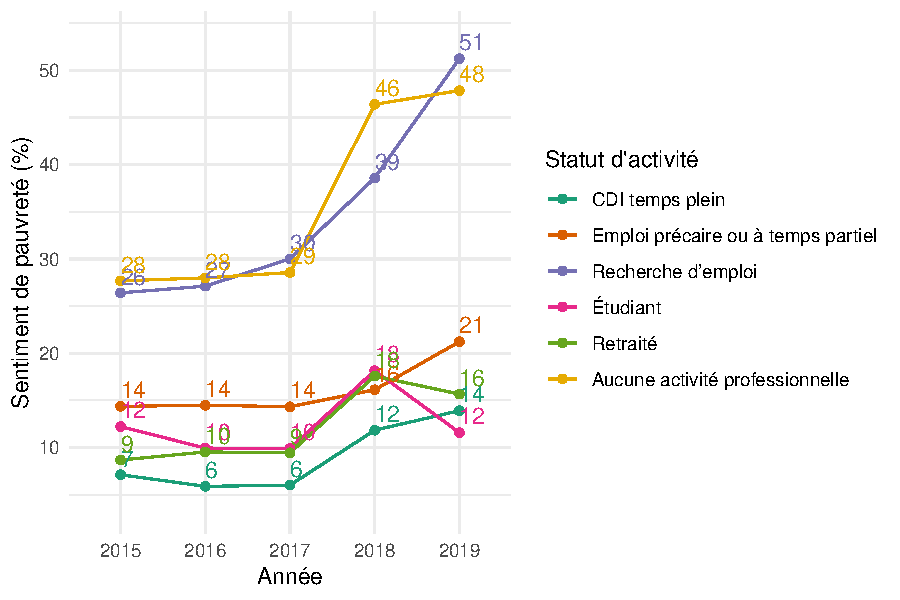
\includegraphics{M2_ANTUNEZ_SQD_files/figure-latex/figstatactevol-1} 

}

\caption{Evolution du sentiment de pauvreté selon le statut d'activité}\label{fig:figstatactevol}
\end{figure}
\begin{note}
\emph{Champ : Personnes d'au moins 18 ans résidant en France métropolitaine.}

\emph{Source : Baromètre d'opinion de la DREES, 2015-2019.}

\end{note}
Au-delà du statut d'activité, le tableau \ref{tab:tabcompa} révèle un effet également de la classe sociale par la significativité positive d'appartenir aux catégories professionnelles d'ouvriers et d'employés. Près d'un ouvrier ou ancien ouvrier sur trois et d'un employé ou ancien employé sur cinq se déclarent pauvre en 2019 (figure \ref{fig:figstatactevol}), avec des écarts qui se creusent avec les autres professions depuis 2015. C'est le cas en particulier pour les ouvriers, dont le coefficient de la régression devient significatif sur la période 2016-2019 alors qu'il ne l'était pas pour la période précédente.
\begin{figure}

{\centering 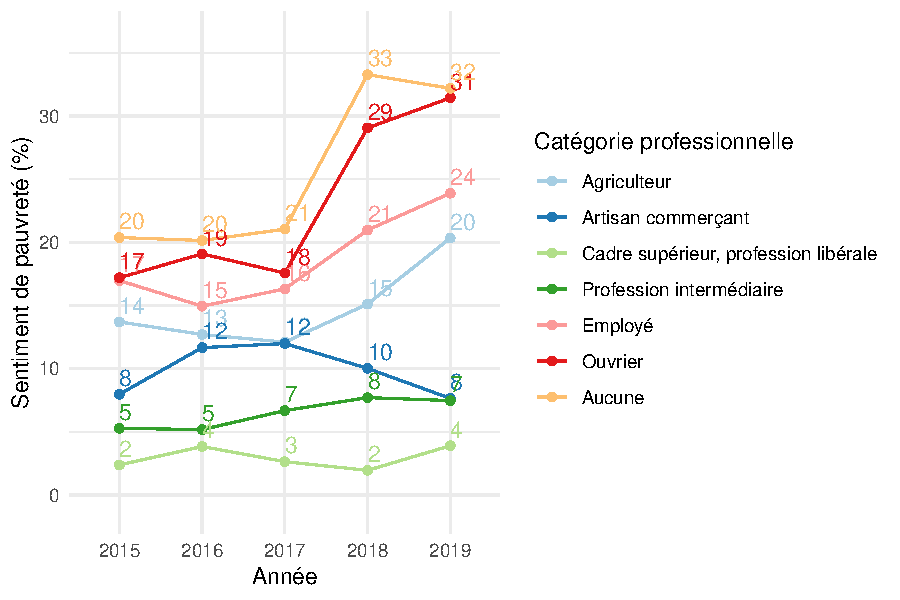
\includegraphics{M2_ANTUNEZ_SQD_files/figure-latex/figpcsevol-1} 

}

\caption{Evolution du sentiment de pauvreté selon la catégorie professionnelle}\label{fig:figpcsevol}
\end{figure}
\begin{note}
\emph{Champ : Personnes d'au moins 18 ans résidant en France métropolitaine.}

\emph{Source : Baromètre d'opinion de la DREES, 2015-2019.}

\end{note}
Le bloc de modalités sur la composition familiale a également beaucoup d'effet sur le sentiment de pauvreté. Le fait de vivre seul(e) joue un rôle déterminant puisqu'il double, toutes les autres variables du modèle étant égales par ailleurs, le risque de se sentir pauvre par rapport à un couple sans enfant (tableau \ref{tab:tabcompa}). Même si le fait d'être le parent d'une famille monoparentale n'est plus significatif en présence des contrôles du modèle, il est la situation familiale qui connaît le plus fort sentiment de pauvreté puisqu'un tiers des personnes dans cette situation se déclarent pauvres (figure \ref{fig:figviefamevol}). Ces résultats semblent illustrer l'effet protecteur du couple sur le fait de se sentir ou non pauvre. Le couple permet en effet notamment de faire des économies d'échelles, notamment en matière de dépenses vis-à-vis de son logement. Au sujet du logement, le fait d'être propriétaire plutôt que locataire diminue significativement les chances de se déclarer pauvre (tableau \ref{tab:tabcompa}).
\begin{figure}

{\centering 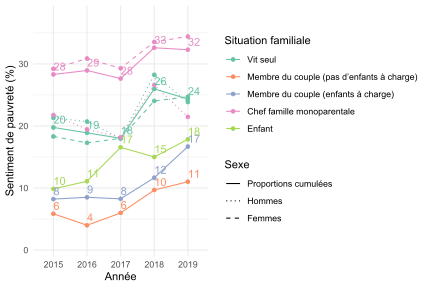
\includegraphics{M2_ANTUNEZ_SQD_files/figure-latex/figviefamevol-1} 

}

\caption{Evolution du sentiment de pauvreté selon la situation familiale}\label{fig:figviefamevol}
\end{figure}
\begin{note}
\emph{Champ : Personnes d'au moins 18 ans résidant en France métropolitaine.}

\emph{Source : Baromètre d'opinion de la DREES, 2015-2019.}

\end{note}
\hypertarget{a-quel-niveau-muxe9nage-individu-se-mesure-la-pauvretuxe9}{%
\subsection{A quel niveau (ménage, individu) se mesure la pauvreté ?}\label{a-quel-niveau-muxe9nage-individu-se-mesure-la-pauvretuxe9}}

L'importance de la structure familiale sur le sentiment de pauvreté invite à s'interroger sur l'échelle de mesure de la pauvreté. Si l'échelle du ménage a son importance (niveau au sein duquel on se partage en général les ressources), il est intéressant d'étudier à quel point l'échelle individuelle joue également.

S'agissant de la mesure de la position sociale, la \emph{dominance approach} (Erikson (1984)) suggère de retenir dans les analyses statistiques uniquement la position sociale (profession ou niveau d'éducation) la plus haute entre deux membres d'un couple, par souci de parcimonie. Dans cette veine, c'est la profession de la personne de référence du ménage qui a longtemps servi de norme en France. Encore aujourd'hui, cette notion est mobilisée dans le Baromètre d'opinion\footnote{Dans le Baromètre, la personne de référence du ménage est définie comme étant la personne interrogée si celle-ci vit seule ou est l'homme du couple du ménage. Elle correspond à l'homme du couple si l'interviewé est une femme, un enfant de la famille ou toute autre personne hébergée par le couple du ménage}, ce qui rend impossible l'étude de la position sociale de l'ensemble du ménage avec cette source de données\footnote{ Le dispositif d'enquête « Statistiques sur les ressources et conditions de vie » (SRCV) serait un outil efficace pour creuser plus en profondeur ces aspects sur la composition du ménage en lien avec la pauvreté (voir partie discussion).}. Les différentes sources de revenus sont, elles, renseignées au niveau du ménage dans le Baromètre.

Or, Cayouette-Remblière \& Ichou (2019) démontrent, grâce à des analyses géométriques des données et classifications réalisées sur deux enquêtes distinctes de la statistique publique\footnote{ Il s'agit de deux enquêtes nationales représentatives : « Trajectoires et origines » (TeO, Ined/Insee, 2008) et le « Panel d'élèves entrant dans le secondaire en 2007 » (DEPP-MEN).}, que tenir compte des configurations familiales permet un pouvoir explicatif supérieur à celui des approches classiques. Depuis peu, des travaux de rénovation de la nomenclature des professions et catégories socioprofessionnelles (PCS) sont d'ailleurs en cours de finalisation dans la statistique publique française (Eidelman \& Chardon (2019)), incluant une « PCS Ménage », permettant d'analyser les inégalités sociales. Il faudra attendre encore quelques années pour que cette approche devienne la norme dans les enquêtes.

Même si les données du Baromètre d'opinion ne sont pas les plus adaptées pour étudier avec précision la composition des ménages et son effet sur la pauvreté, elles permettent toutefois d'observer, en interrogeant les Français sur plusieurs niveaux de perception du RSA (soi-même, au sein du ménage, au sein de la famille, et dans son entourage), que chaque niveau a son influence (coefficients significatifs dans le tableau \ref{tab:tabrsa}) sur le sentiment de pauvreté, le niveau individuel ayant celui qui a le plus gros effet.
\begin{table}

\caption{\label{tab:tabrsa}Mesure de l'effet d'être bénéficiaire du RSA à différents niveaux (individu, ménage et entourage) sur le sentiment de pauvreté}
\centering
\begin{tabular}[t]{>{\raggedright\arraybackslash}p{6cm}>{\raggedright\arraybackslash}p{2cm}}
\toprule
Modèle logit. Variable dépendante : se déclarer pauvre & Odds ratio\\
\midrule
\addlinespace[0.3em]
\multicolumn{2}{l}{\textbf{Individu}}\\
\hspace{1em}N'est pas une personne au RSA & Réf.\\
\hspace{1em}Est une personne au RSA & 4,65***\\
\addlinespace[0.3em]
\multicolumn{2}{l}{\textbf{Ménage}}\\
\hspace{1em}N'a personne dans son ménage au RSA & Réf.\\
\hspace{1em}A quelqu'un dans son ménage au RSA & 2,62***\\
\addlinespace[0.3em]
\multicolumn{2}{l}{\textbf{Famille}}\\
\hspace{1em}Ne connaît personne dans sa famille au RSA & Réf.\\
\hspace{1em}Connaît quelqu'un dans sa famille au RSA & 1,55***\\
\addlinespace[0.3em]
\multicolumn{2}{l}{\textbf{Hors famille}}\\
\hspace{1em}Ne connaît personne hors famille au RSA & Réf.\\
\hspace{1em}Connaît quelqu'un hors famille au RSA & 1,59***\\
\bottomrule
\multicolumn{2}{l}{\rule{0pt}{1em}\textit{Note: }}\\
\multicolumn{2}{l}{\rule{0pt}{1em}N = 11628 et \$R\textasciicircum{}2\$ ajusté = 5,9 \%.}\\
\multicolumn{2}{l}{\rule{0pt}{1em}* : significatif au seuil de 5 \% ; ** : 1 \% ; *** : 0,1 \%.}\\
\end{tabular}
\end{table}
\begin{note}
\emph{Champ : Personnes d'au moins 18 ans résidant en France métropolitaine.}

\emph{Source : Baromètre d'opinion de la DREES, 2016-2019.}

\emph{Lecture : Entre 2016 et 2019, toutes les autres variables de cette régression étant égales par ailleurs, le risque pour une personne dont le ménage est bénéficiaire du RSA de se déclarer pauvre plutôt que le contraire est 2,62 fois celui d'une personne non bénéficiaire.}

\end{note}
\hypertarget{quelles-variables-du-baromuxe8tre-intuxe9grer-dans-les-dimensions-monuxe9taire-et-institutionnelle-de-la-pauvretuxe9}{%
\subsection{Quelles variables du Baromètre intégrer dans les dimensions monétaire et institutionnelle de la pauvreté ?}\label{quelles-variables-du-baromuxe8tre-intuxe9grer-dans-les-dimensions-monuxe9taire-et-institutionnelle-de-la-pauvretuxe9}}

Duvoux \& Papuchon (2018) ont ainsi montré que la pauvreté monétaire, mesurée par le quintile de niveau de vie du ménage des individus, n'est pas l'unique facteur explicatif du sentiment de pauvreté. Même à quintile de niveau de vie fixé, la pauvreté institutionnelle -- mesurée par le fait d'être bénéficiaire du RSA, d'allocations chômage ou de prestations liées au handicap, à l'invalidité ou à la dépendance -- et d'autres caractéristiques sociodémographiques telles que le statut d'emploi, la profession et la composition du ménage, ont également un effet sur le sentiment de pauvreté.

S'agissant de la dimension monétaire de la pauvreté, le quintile de niveau de vie n'est pas la seule variable mobilisable dans le Baromètre. C'est pourquoi nous avons testé l'effet sur le sentiment de pauvreté de recevoir différents types de revenus (salaires, activité indépendante, retraite, actifs financiers et locations). Si tous les coefficients sont bien significatifs, tous les types de revenus étant égaux par ailleurs (tableau \ref{tab:tabmon}), nous ne conservons dans les prochains modèles que les revenus de locations et d'actifs qui ont les odds-ratio les plus élevés et sont les seuls qui demeurent significatifs quand on ajoute le statut d'activité et la PCS en variables de contrôles.
\begin{table}

\caption{\label{tab:tabmon}Mesure de l'effet de la pauvreté monétaire sur le sentiment de pauvreté}
\centering
\begin{tabular}[t]{>{\raggedright\arraybackslash}p{6cm}>{\raggedright\arraybackslash}p{2cm}}
\toprule
Modèle logit. Variable dépendante : se déclarer pauvre & Odds ratio\\
\midrule
Quintile 1 & 1,72***\\
Quintile 2 & Réf.\\
Quintile 3 & 0,4***\\
Quintile 4 & 0,17***\\
Quintile 5 & 0,09***\\
\addlinespace
Pas de revenus de salaires & Réf.\\
Revenus de salaires & 0,52***\\
Pas de revenus d'activité indépendante & Réf.\\
Revenus d'activité indépendante & 0,49***\\
Pas de revenus de retraite & Réf.\\
\addlinespace
Revenus de retraite & 0,6***\\
Pas de revenus d'actifs financiers & Réf.\\
Revenus d'actifs financiers & 0,35***\\
Pas de revenus de locations & Réf.\\
Revenus de locations & 0,17***\\
\bottomrule
\multicolumn{2}{l}{\rule{0pt}{1em}\textit{Note: }}\\
\multicolumn{2}{l}{\rule{0pt}{1em}N = 10817 et \$R\textasciicircum{}2\$ ajusté = 18,5 \%.}\\
\multicolumn{2}{l}{\rule{0pt}{1em}* : significatif au seuil de 5 \% ; ** : 1 \% ; *** : 0,1 \%.}\\
\end{tabular}
\end{table}
\begin{note}
\emph{Champ : Personnes d'au moins 18 ans résidant en France métropolitaine.}

\emph{Source : Baromètre d'opinion de la DREES, 2016-2019.}

\end{note}
S'agissant de la pauvreté institutionnelle, le contour choisi est un peu plus large que Duvoux \& Papuchon (2018) afin d'utiliser un maximum de données empiriques présentes dans le Baromètre. En plus du RSA, des allocations chômage et des prestations liées au handicap, à l'invalidité ou à la dépendance, nous étudions l'effet de la perception des APL\footnote{Duvoux \& Papuchon (2018) placent les APL à part en indiquant que « {[}Même si{]} ces allocations sont versées sous conditions de ressources, {[}\ldots{]} {[}elles{]} n'impliquent pas de relation étroite avec les services de l'Etat. »}, le fait d'être locataire d'un logement social ou de recevoir au sein de son ménage une bourse d'étude. A part les bourses d'études, les autres prestations sociales ont un effet significatif et positif sur le fait de se sentir pauvre (tableau \ref{tab:tabinst}) et l'effet est particulièrement fort s'agissant du RSA et des APL.
\begin{table}

\caption{\label{tab:tabinst}Mesure de l'effet de la pauvreté institutionnelle sur le sentiment de pauvreté}
\centering
\begin{tabular}[t]{>{\raggedright\arraybackslash}p{6cm}>{\raggedright\arraybackslash}p{2cm}}
\toprule
Modèle logit. Variable dépendante : se déclarer pauvre & Odds ratio\\
\midrule
Pas de RSA & Réf.\\
RSA & 2,79***\\
Pas d'allocation chômage & Réf.\\
Allocation chômage & 1,38***\\
Pas d'APL & Réf.\\
\addlinespace
APL & 3,37***\\
Pas d'AAH, APA, PCH (handicap) & Réf.\\
AAH, APA, PCH (handicap) & 1,41***\\
Pas de bourse d'étude & Réf.\\
bourse d'étude & 0,84\\
\addlinespace
Locataire privé / hébergé, Propriétaire & Réf.\\
Locataire HLM & 1,89***\\
\bottomrule
\multicolumn{2}{l}{\rule{0pt}{1em}\textit{Note: }}\\
\multicolumn{2}{l}{\rule{0pt}{1em}N = 11630 et \$R\textasciicircum{}2\$ ajusté = 12,5 \%.}\\
\multicolumn{2}{l}{\rule{0pt}{1em}* : significatif au seuil de 5 \% ; ** : 1 \% ; *** : 0,1 \%.}\\
\end{tabular}
\end{table}
\begin{note}
\emph{Champ : Personnes d'au moins 18 ans résidant en France métropolitaine.}

\emph{Source : Baromètre d'opinion de la DREES, 2016-2019.}

\end{note}
Le tableau \ref{tab:tabfinal21} présente une dernière modélisation économétrique du sentiment de pauvreté. Par souci de parcimonie du modèle, nous proposons une seule variable rassemblant statut d'activité et PCS, retirant ainsi quelques modalités non significatives précédemment. Nous y ajoutons en revanche des variables supplémentaires : les quelques variables additionnelles de pauvreté monétaire et institutionnelle évoquées dans les deux paragraphes précédents, une indicatrice de si l'individu se considère comme étant en emploi précaire (qui est positivement significative\footnote{Contrairement aux mesures d'emploi précaire basées uniquement sur le temps partiel et type de contrat, cf.~tableau \ref{tab:tabcompa}.}) et également une indicatrice intégrant le fait d'avoir dans ses proches quelqu'un au RSA (également positivement significative à 5 \%). Dans ce nouveau modèle, l'effet du diplôme ressort davantage et est peut-être dû à la simplification des modalités concernant la situation professionnelle. Le fait d'être chômeur a un effet au-delà même du fait de recevoir une prestation chômage. Les prestations liées au handicap et au fait d'être locataire d'un logement social ne ressortent plus significatives. Pour cette dernière modalité cela est dû au fait qu'elle reste proche du fait d'être locataire du privé. Enfin, l'effet de la structure familial est semblable à précédemment, avec, en particulier, un effet amplificateur du fait de vivre seul sur le sentiment de pauvreté.
\begin{longtable}[t]{>{\raggedright\arraybackslash}p{4cm}>{\raggedright\arraybackslash}p{6cm}>{\raggedright\arraybackslash}p{4cm}}
\caption{\label{tab:tabfinal21}Modèle de synthèse des effets sur le sentiment de pauvreté}\\
\toprule
Modèle logit & Variable dépendante : se déclarer pauvre & Odds ratio\\
\midrule
\endfirsthead
\caption[]{\label{tab:tabfinal21}Modèle de synthèse des effets sur le sentiment de pauvreté \textit{(suite)}}\\
\toprule
Modèle logit & Variable dépendante : se déclarer pauvre & Odds ratio\\
\midrule
\endhead
\midrule
\multicolumn{3}{r@{}}{\textit{(suite en page suivante...)}}\
\endfoot
\bottomrule
\multicolumn{3}{l}{\rule{0pt}{1em}\textit{Note: }}\\
\multicolumn{3}{l}{\rule{0pt}{1em}N = 10726 et \$R\textasciicircum{}2\$ ajusté = 26,6 \%.}\\
\multicolumn{3}{l}{\rule{0pt}{1em}* : significatif au seuil de 5 \% ; ** : 1 \% ; *** : 0,1 \%.}\\
\endlastfoot
\addlinespace[0.3em]
\multicolumn{3}{l}{\textbf{Pauvreté monétaire}}\\
\hspace{1em}Niveau de vie & Quintile 1 & 1,48***\\
\hspace{1em} & Quintile 2 & Réf.\\
\hspace{1em} & Quintile 3 & 0,52***\\
\hspace{1em} & Quintile 4 & 0,25***\\
\hspace{1em} & Quintile 5 & 0,18***\\
\hspace{1em}Types de ressources & Pas de revenus de locations & Réf.\\
\hspace{1em}perçues par le ménage & Revenus de locations & 0,23***\\
\hspace{1em}(12 mois) & Pas de revenus d'actifs financiers & Réf.\\
\hspace{1em} & Revenus d'actifs financiers & 0,47**\\
\addlinespace[0.3em]
\multicolumn{3}{l}{\textbf{Pauvreté institutionnelle}}\\
\hspace{1em} & Pas de RSA & Réf.\\
\hspace{1em} & RSA & 1,98***\\
\hspace{1em} & Pas d'APL & Réf.\\
\hspace{1em} & APL & 1,62***\\
\hspace{1em} & Pas d'allocation chômage & Réf.\\
\hspace{1em} & Allocation chômage & 1,28**\\
\hspace{1em} & Pas d'AAH, APA, PCH (handicap) & Réf.\\
\hspace{1em} & AAH, APA, PCH (handicap) & 1,07\\
\hspace{1em}Logement & Locataire HLM & 1,02\\
\addlinespace[0.3em]
\multicolumn{3}{l}{\textbf{Contrôles}}\\
\hspace{1em} & Locataire privé / hébergé & Réf.\\
\hspace{1em} & Propriétaire & 0,47***\\
\hspace{1em}Situation professionnelle & Agriculteur & 2,94*\\
\hspace{1em} & Artisan commerçant & 0,62\\
\hspace{1em} & Cadre supérieur, profession libérale & 0,57*\\
\hspace{1em} & Profession intermédiaire & Réf.\\
\hspace{1em} & Employé & 1,45*\\
\hspace{1em} & Ouvrier & 1,59**\\
\hspace{1em} & Chômeur & 1,6**\\
\hspace{1em} & Retraité & 1,45\\
\hspace{1em} & Au foyer & 1,56*\\
\hspace{1em} & Autre inactif & 1,85***\\
\hspace{1em}Précarité de l'emploi & N'est pas personne en emploi précaire & Réf.\\
\hspace{1em}(subjective) & est personne en emploi précaire & 1,4**\\
\hspace{1em}Niveau de diplôme le plus élevé & CAP, BEP ou moins & 1,24*\\
\hspace{1em} & Baccalauréat & Réf.\\
\hspace{1em} & Bac + 2 & 0,73*\\
\hspace{1em} & Bac + 3 ou plus & 0,68**\\
\hspace{1em}Classe d'âge & 18 à 29 ans & 0,52***\\
\hspace{1em} & 30 à 39 ans & Réf.\\
\hspace{1em} & 40 à 49 ans & 1,01\\
\hspace{1em} & 50 à 59 ans & 0,91\\
\hspace{1em} & 60 à 69 ans & 0,96\\
\hspace{1em} & 70 ans et plus & 0,76\\
\hspace{1em}Situation familiale & Vit seul & 1,7***\\
\hspace{1em} & Membre du couple (pas d’enfants à charge) & Réf.\\
\hspace{1em} & Membre du couple (enfants à charge) & 0,7**\\
\hspace{1em} & Chef famille monoparentale & 1,26\\
\hspace{1em} & Enfant & 1,1\\
\hspace{1em} & Autre situation familiale & 1,43\\
\hspace{1em}Sexe & Femme & Réf.\\
\hspace{1em} & Homme & 1,14\\
\hspace{1em}Entourage au RSA & Ne connaît pas de personne au RSA & Réf.\\
\hspace{1em} & Connait une personne au RSA & 1,16*\\
\hspace{1em}Année & 2016 & Réf.\\
\hspace{1em} & 2017 & 1,03\\
\hspace{1em} & 2018 & 1,97***\\
\hspace{1em} & 2019 & 2,22***\\*
\end{longtable}
\begin{note}
\emph{Champ : Personnes d'au moins 18 ans résidant en France métropolitaine.}

\emph{Source : Baromètre d'opinion de la DREES, 2016-2019.}

\end{note}
\hypertarget{sec:traducsp}{%
\section{Que peut traduire le sentiment de pauvreté ?}\label{sec:traducsp}}

Pauvreté objective (monétaire et institutionnelle) mais aussi : insécurité sociale, déclassement, pessimisme\ldots{}

ME1 filtre : non 2018
Pensez-vous pouvoir compter sur quelqu'un en cas de grave problème personnel ?
1. Oui, certainement
2. Oui, probablement
3. Non probablement pas
4. Non, certainement pas
5. {[}NSP{]}

ME2 filtre : non 2018
Compte tenu de vos ressources, diriez-vous que votre ménage a des difficultés pour boucler ses
fins de mois \ldots{} ?
1. Souvent
2. De temps en temps
3. Rarement
4. Jamais
5. {[}NSP{]}

ME3 Filtre : non 2018
En imaginant que vous deviez faire face à une dépense imprévue de 500 € dans l'année qui vient,
pensez-vous\ldots{} ?
1. Que vous y feriez face sans trop de problème
2. Qu'il vous serait assez difficile d'y faire face
3. Qu'il vous serait très difficile d'y faire face
4. {[}NSP{]}

ME4 filtre : non 2018
Êtes-vous inquiet.e à l'idée de ne pas pouvoir être bien soigné en cas de gros problème de santé ?
1. Oui, très inquiet.e
2. Oui, assez inquiet.e
3. Non, pas très inquiet.e
4. Non, pas inquiet.e du tout
5. {[}NSP{]}

ME5 filtre : non 2018
Globalement, diriez-vous que les revenus de votre foyer sont plutôt variables ou plutôt stables d'un
mois sur l'autre ?
1. Plutôt stables
2. Plutôt variables
3. {[}NSP{]}

ME6 filtre : non 2018
Dans les mois qui viennent, pensez-vous que les revenus de votre foyer vont\ldots{} ?
1. Plutôt augmenter
2. Plutôt diminuer
3. Rester stables
4. {[}NSP{]}
\begin{center}\rule{0.5\linewidth}{0.5pt}\end{center}

OG1 filtre : non SOCLE 2002-
Vous personnellement, comment qualifieriez-vous votre situation actuelle ? Diriez-vous de votre situation actuelle, qu'elle est \ldots{}
1. Très bonne
2. Assez bonne
3. Assez mauvaise
4. Très mauvaise
5. {[}NSP{]}

OG2 filtre : non SOCLE 2017 -
Par rapport à la situation de vos parents au même âge, diriez-vous que votre situation actuelle est\ldots{} ?
1. Bien meilleure
2. Plutôt meilleure
3. À peu près identique
4. Plutôt moins bonne
5. Bien moins bonne
6. {[}NSP{]}

OG3 filtre : non SOCLE 2000 -
Quand vous pensez à l'avenir, êtes-vous plutôt optimiste ou plutôt pessimiste\ldots{} ?
1. Très optimiste
2. Plutôt optimiste
3. Plutôt pessimiste
4. Très pessimiste
5. {[}NSP{]}
\_1 Pour vous-même
\_2 Pour vos enfants ou les générations futures

OG4 filtre : non SOCLE 2000 -
Pour chacun des sujets suivants, dites-moi s'il VOUS préoccupe VOUS PERSONNELLEMENT beaucoup, assez, peu ou pas du tout ?
1. Beaucoup
2. Assez
3. Peu
4. Pas du tout
5. {[}NSP{]}

ENQUETEUR : MONTRER L'ÉCRAN ET ENUMERER

\_1 Le logement 2014 -
\_2 Les migrations des populations des pays pauvres vers les pays riches
\_3 La pauvreté
\_4 L'insécurité dans votre quartier ou votre village 2014 -
\_5 La dette de la France 2014 -
\_6 Le chômage
\_7 Les crises financières internationales
\_8 La santé des Français 2014 -
\_9 le niveau des salaires et du pouvoir d'achat 2014 -

ROTATION ALEATOIRE

OG5 filtre : non
Et pour les sujets suivants, dites-moi s'il VOUS préoccupe VOUS PERSONNELLEMENT beaucoup, assez, peu ou pas du tout ?
1. Beaucoup
2. Assez
3. Peu
4. Pas du tout
5. {[}NSP{]}

ENQUETEUR : MONTRER ECRAN ET ENUMERER

\_1 Les problèmes liés à l'environnement 2000 -
\_2 Les risques alimentaires 2000 -- 2018 ; MODULE ANNEE IMPAIRE 2019 -
\_3 Le Sida 2000 -- 2018 ; MODULE ANNEE IMPAIRE 2019 -
\_4 L'avenir du système de retraite 2014 --
\_5 Le cancer 2000 -
\_6 Les risques d'épidémie 2009 -- 2018 ; MODULE ANNEE IMPAIRE 2019 -
\_7 Les inégalités entre les femmes et les hommes 2014 --

IN1 filtre : non SOCLE 2000 -
La société française aujourd'hui, vous paraît-elle plutôt juste ou plutôt injuste ?
1. Plutôt juste
2. Plutôt injuste
3. {[}NSP{]}

IN2 filtre : non SOCLE 2000 -
Globalement, depuis 5 ans, diriez-vous que les inégalités en France\ldots{} ?
1. Ont plutôt augmenté
2. Ont plutôt diminué
3. {[}Sont restées stables{]}
4. {[}NSP{]}

IN3 filtre : non SOCLE 2000 -
Et à l'avenir, pensez-vous que les inégalités en France\ldots{} ?
1. Vont plutôt augmenter
2. Vont plutôt diminuer
3. {[}Resteront stables{]}
4. {[}NSP{]}

IN11filtrer si : si SDACT \textless{} 5 SOCLE 2014 -
\emph{1 Que gagnent en moyenne les gens qui ont la même profession que vous ?
\_}\_\_\_\_\_\_\_\_/
\emph{2 Que devraient gagner en moyenne les gens qui ont la même profession que vous ?
\_}\_\_\_\_\_\_\_\_/
ENQUÊTEUR : POSEZ LA QUESTION POUR LA DERNIÈRE PROFESSION EXERCÉE SI RETRAITÉ OU CHOMEUR AYANT DÉJÀ TRAVAILLE. NOTEZ LE SALAIRE (OU LA RÉMUNÉRATION) NET(TE) MENSUEL(LE) EN EUROS. SI L'ENQUÊTÉ RÉPOND EN FRANCS, TRADUIRE EN EUROS. NOTEZ 999 999 999 POUR « NE SAIT PAS » (OU REFUS DE RÉPONDRE). SI L'ENQUÊTÉ TRAVAILLE À MI-TEMPS, CONVERTIR EN PLEIN TEMPS.
CODAGE : QUANTITÉ

PE1 Filtre : non SOCLE 2000 -
Selon vous, depuis 5 ans, la pauvreté et l'exclusion en France\ldots{}
1. Ont diminué
2. Ont augmenté
3. {[}Sont restées stables{]}
4. {[}NSP{]}
ENQUETEUR : ENUMERER
PE2 Filtre : non SOCLE 2000 -
Et à l'avenir, pensez-vous que la pauvreté et l'exclusion en France\ldots{} ?
1. Vont plutôt diminuer
2. Vont plutôt augmenter
3. {[}Resteront stables{]}
4. {[}NSP{]}
ENQUETEUR : ENUMERER

\hypertarget{limportante-prise-en-compte-du-risque-de-pauvretuxe9-subjectif}{%
\section{L'importante prise en compte du risque de pauvreté subjectif}\label{limportante-prise-en-compte-du-risque-de-pauvretuxe9-subjectif}}

\hypertarget{espace-social-des-pauvretuxe9s-monuxe9taire-institutionelle-et-subjective-par-analyse-des-correspondances-multiples}{%
\subsection{Espace social des pauvretés monétaire institutionelle et subjective par Analyse des Correspondances Multiples}\label{espace-social-des-pauvretuxe9s-monuxe9taire-institutionelle-et-subjective-par-analyse-des-correspondances-multiples}}
\begin{figure}

{\centering 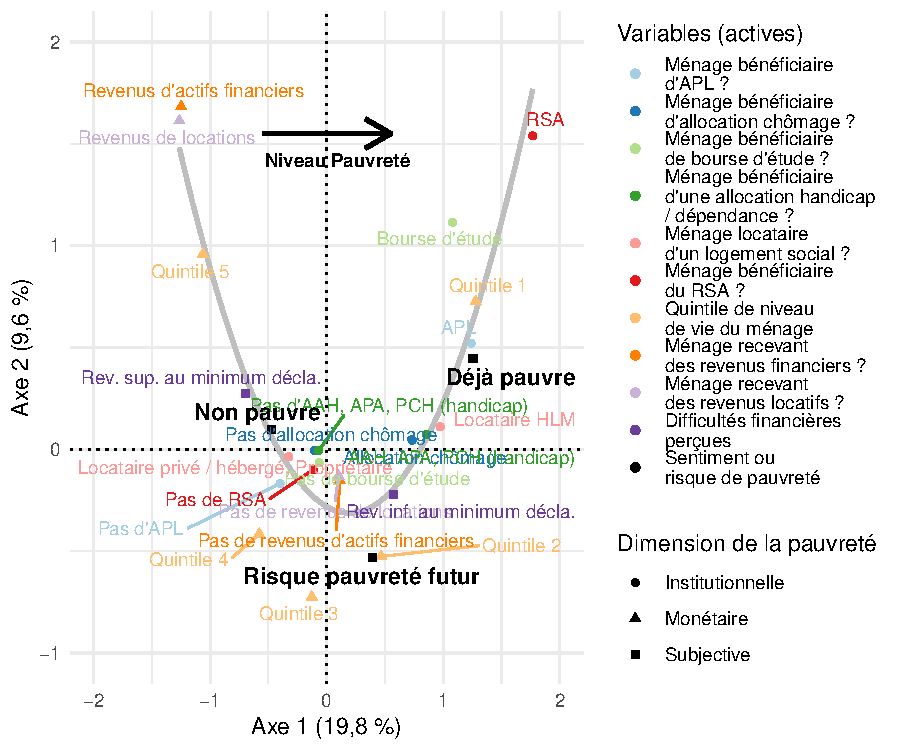
\includegraphics{M2_ANTUNEZ_SQD_files/figure-latex/acm1-1} 

}

\caption{ACM}\label{fig:acm1}
\end{figure}
\hypertarget{la-pauvretuxe9-subjective-en-trois-modalituxe9s-absence-pruxe9sence-et-risque-uxe0-venir}{%
\subsection{La pauvreté subjective en trois modalités : absence, présence et risque à venir}\label{la-pauvretuxe9-subjective-en-trois-modalituxe9s-absence-pruxe9sence-et-risque-uxe0-venir}}

\hypertarget{la-pauvretuxe9-comme-dimension-latente}{%
\section{La pauvreté comme dimension latente}\label{la-pauvretuxe9-comme-dimension-latente}}

\hypertarget{comment-moduxe9liser-des-variables-latentes}{%
\subsection{Comment modéliser des variables latentes ?}\label{comment-moduxe9liser-des-variables-latentes}}

\hypertarget{construction-dun-espace-social-par-analyse-factorielle}{%
\subsection{Construction d'un espace social par analyse factorielle}\label{construction-dun-espace-social-par-analyse-factorielle}}

\hypertarget{conclusion-discussion}{%
\chapter*{Conclusion / Discussion}\label{conclusion-discussion}}
\addcontentsline{toc}{chapter}{Conclusion / Discussion}

\appendix

\hypertarget{annexequestio}{%
\chapter{Extraits du questionnaire du Baromètre d'opinion}\label{annexequestio}}

\hypertarget{pauvretuxe9-monuxe9taire}{%
\section{Pauvreté monétaire}\label{pauvretuxe9-monuxe9taire}}

\textbf{SDREVCL} \emph{filtre : non} SOCLE 2012 -

Nous désirons analyser les résultats de cette étude en fonction des revenus familiaux des personnes que nous avons interrogées.
Nous désirons savoir à quel niveau de revenus MENSUELS NETS AVANT IMPOTS se situe votre foyer en comptant {[}réponses en SDRES{]}.

\emph{CODAGE : DONNER ICI DANS LE CORPS DE LA QUESTION LA LISTE DU TYPE DE RESSOURCES QUE LES PERSONNES ONT DIT PERCEVOIR EN SDRES.}

/\_ \_ \_ \_ \_ \_ \_ /

\emph{ENQUETEUR : NOTER EN CLAIR - SI BESOIN PRECISER : NOUS NOUS INTERESSONS A L'ENSEMBLE DES RESSOURCES DU MENAGE, Y COMPRIS CELLES DE VOTRE CONJOINT, DE VOS ENFANTS, ETC. SI REFUS DE REPONDRE NOTER 999 999 999 EUROS NETS PAR MOIS}

\emph{Remarque : avant 2012, les enquêtés ne sont interrogés que sur des tranches de revenu.}
\begin{center}\rule{0.5\linewidth}{0.5pt}\end{center}

\textbf{SDREVTR} \emph{filtre : si refus de répondre à SDREVCL} SOCLE 2000 -

A défaut de me préciser un montant, pourriez-vous me dire dans quelle tranche vous vous situez dans l'échelle de revenus MENSUELS NETS AVANT IMPOTS DE L'ENSEMBLE DE VOTRE FOYER que je vais vous citer ? Je vous parle bien des revenus de toute la famille.
\begin{enumerate}
\def\labelenumi{\arabic{enumi}.}
\tightlist
\item
  A. Moins de 1000 euros par mois\\
\item
  B. De 1000 à moins de 1400 euros par mois\\
\item
  C. De 1400 à moins de 1900 euros par mois
\item
  D. De 1900 à moins de 2400 euros par mois\\
\item
  E. De 2400 à moins de 3800 euros par mois
\item
  F. De 3800 à moins de 5300 euros par mois
\item
  G. Plus de 5300 euros par mois
\item
  {[}NSP/refus de réponse{]}
\end{enumerate}
\emph{ENQUETEUR : MONTRER LA CARTE REPONSE OBLIGATOIREMENT -- DEMANDER LA LETTRE QUI CORRESPOND A LA TRANCHE DE REVENUS}

\hypertarget{pauvretuxe9-institutionnelle-monuxe9taire}{%
\section{Pauvreté institutionnelle / monétaire}\label{pauvretuxe9-institutionnelle-monuxe9taire}}

\textbf{SDRES} \emph{filtre : non} SOCLE 2000 -

Au cours des douze derniers mois, votre ménage a-t-il perçu des ressources provenant de\ldots{}
\begin{enumerate}
\def\labelenumi{\arabic{enumi}.}
\tightlist
\item
  Oui
\item
  Non
\item
  {[}NSP{]}
\end{enumerate}
\begin{itemize}
\tightlist
\item
  \_1 Salaires, traitements et primes
\item
  \_2 Revenus d'une activité professionnelle indépendante
\item
  \_3 RSA (Revenu de solidarité active)
\item
  \_4 Allocations de chômage
\item
  \_5 Préretraite, retraites
\item
  \_6 Revenus d'actifs financiers
\item
  \_7 Revenus de locations
\item
  \_8 Prestations familiales (allocations familiales, complément familial, prestation d'accueil du jeune enfant (PAJE)\ldots) 2013 -
\item
  \_9 Allocations de logement (APL, \ldots)
\item
  \_10 Prestations liées au handicap, à l'invalidité ou à la dépendance (AAH, APA, PCH\ldots) 2013 -
\item
  \_11 Bourses d'études 2015 -
\item
  \_12 Pensions alimentaires ou argent reçu tous les mois de la part de proches (familles, amis\ldots) 2015 -
  Remarque : en 2013, les AL ont été séparées des prestations familiales
\end{itemize}
\hypertarget{pauvretuxe9-subjective-1}{%
\section{Pauvreté subjective}\label{pauvretuxe9-subjective-1}}

\textbf{PE3} \emph{filtre : non} SOCLE 2014 -

Et vous personnellement, pensez-vous qu'il y a un risque que vous deveniez pauvre dans les cinq prochaines années ?
\begin{enumerate}
\def\labelenumi{\arabic{enumi}.}
\tightlist
\item
  Oui, plutôt
\item
  Non, plutôt pas
\item
  Je me considère déjà comme pauvre
\item
  {[}NSP{]}
\end{enumerate}
\emph{ENQUETEUR : ENUMERER - UNE SEULE REPONSE}
\begin{center}\rule{0.5\linewidth}{0.5pt}\end{center}

\textbf{PE16} \emph{filtre : non} SOCLE 2014 -

Selon vous, pour vivre, quel est le montant dont doit disposer AU MINIMUM un foyer comme le vôtre, par mois (en euros) ?

\emph{ENQUETEUR : SI BESOIN, PRECISER, EN EUROS NETS. SI NSP OU REFUS DE REPONDRE CODER 999 999 999.}

\emph{CODAGE : QUANTITE}
\begin{center}\rule{0.5\linewidth}{0.5pt}\end{center}

\textbf{PE15} \emph{filtre : non} MODULE ANNEES PAIRES 2014 -

Actuellement, compte tenu de votre situation globale, du montant des aides publiques (RSA, allocations familiales, aides au logement), et du montant de vos impôts, vous considérez que :
\begin{enumerate}
\def\labelenumi{\arabic{enumi}.}
\tightlist
\item
  Vous êtes suffisamment aidé.e par les pouvoirs publics, ou n'avez pas besoin d'être aidé.e
\item
  Vous auriez besoin d'être aidé.e davantage par les pouvoir publics
\item
  {[}Non concerné.e{]}
\item
  {[}NSP{]}
\end{enumerate}
\emph{ENQUETEUR : MONTRER ECRAN ET ENUMERER - UNE SEULE REPONSE}

\hypertarget{socioduxe9mographie}{%
\section{Sociodémographie}\label{socioduxe9mographie}}

\textbf{SDSEXE} \emph{filtre : non} SOCLE 2000-

Sexe de l'enquêté.e

\emph{ENQUETEUR : L'INTERVIEWE EST UN HOMME OU UNE FEMME ?}
\begin{enumerate}
\def\labelenumi{\arabic{enumi}.}
\tightlist
\item
  Un homme
\item
  Une femme
\end{enumerate}
\begin{center}\rule{0.5\linewidth}{0.5pt}\end{center}

\textbf{SDANNAIS} \emph{filtre : non} SOCLE 2000-

Tout d'abord, pouvez-vous m'indiquer votre année de naissance :

\emph{Remarque : âge minimum de 18 ans.}
\begin{center}\rule{0.5\linewidth}{0.5pt}\end{center}

\textbf{SDAGE} \emph{filtre : non} SOCLE 2000-

\emph{RECODAGE DE SDANNAIS}
\begin{center}\rule{0.5\linewidth}{0.5pt}\end{center}

\textbf{SDSITUA} \emph{filtre : non} SOCLE 2000-

Quelle est votre situation actuellement ?
\begin{enumerate}
\def\labelenumi{\arabic{enumi}.}
\tightlist
\item
  Vous travaillez à temps plein
\item
  Vous travaillez à temps partiel
\item
  Vous travaillez de façon intermittente
\item
  Vous êtes à la recherche d'un emploi (y compris au chômage)
\item
  Vous êtes étudiant.e
\item
  Vous êtes retraité.e ou préretraité.e
\item
  Vous n'exercez aucune activité professionnelle
\end{enumerate}
\emph{Remarque : avant 2014, l'ensemble des inactifs (étudiant, retraité, aucune activité professionnelle) était regroupé dans une seule modalité, la modalité 8.}
\begin{center}\rule{0.5\linewidth}{0.5pt}\end{center}

\textbf{SDACT} \emph{filtre : non} SOCLE 2014 -

Quelle est (était) votre activité principale :
\begin{enumerate}
\def\labelenumi{\arabic{enumi}.}
\tightlist
\item
  Salarié.e du secteur privé
\item
  Salarié.e du secteur public
\item
  Indépendant.e sans salarié
\item
  Indépendant.e employeur.euse
\item
  A la recherche d'un premier emploi
\item
  Élève, étudiant.e, en formation, ou en stage non rémunéré
\item
  Apprenti.e sous contrat ou stagiaire rémunéré.e
\item
  Au foyer
\item
  Autre inactif
\end{enumerate}
\emph{CODAGE : SI SDSITUA = 4 OU 6, POSER LA QUESTION SDACT AVEC « ETAIT » AU LIEU DE « EST ».}
\begin{center}\rule{0.5\linewidth}{0.5pt}\end{center}

\textbf{SDSTAT} \emph{filtre : non} SOCLE 2000 -

Question non posée, recodage du statut d'activité de la personne interrogée
\begin{enumerate}
\def\labelenumi{\arabic{enumi}.}
\tightlist
\item
  Salarié.e du secteur public
\item
  Salarié.e du secteur privé
\item
  Indépendant.e sans salarié
\item
  Employeur.euse
\item
  Chômeur.euse
\item
  Inactif.ive
\item
  Autre
\item
  {[}NSP{]}
\end{enumerate}
\emph{RECODAGE : A PARTIR DE SDSITUA ET SDACT}

\emph{Remarque : jusqu'en 2013, cette question était posée directement aux enquêtés.}
\begin{center}\rule{0.5\linewidth}{0.5pt}\end{center}

\textbf{SDPROF} \emph{filtre : filtrer si SDSITUA = 7} SOCLE 2000-

Quelle est (était) votre profession ?

\emph{ENQUETEUR : NOTER EN CLAIR - NOTER LE MAXIMUM DE PRECISIONS}

\emph{CODAGE : EN PRINCIPE SDSITUA PERMET DE REPÉRER LES ACTIFS OCCUPÉS (1 À 3), LES CHÔMEURS (4) ET LES RETRAITÉS (6). SI SDSITUA = 4 OU 6, POSER LA QUESTION AVEC « ETAIT » AU LIEU DE « EST ».}

\emph{VARIABLE NON DIFFUSEE}
\begin{center}\rule{0.5\linewidth}{0.5pt}\end{center}

\textbf{SDPCS7} \emph{filtre : non} SOCLE 2000 -

\emph{ENQUETEUR : CODER LA PROFESSION DE L'INTERVIEWE (SUR LES 7 CATEGORIES SOCIO-PROFESSIONNELLES QUI SUIVENT), SI CHOMEUR OU RETRAITE CODER SON ANCIENNE PROFESSION (C'EST LA REPONSE EN CLAIR A SDPROF DANS SON INTEGRALITE QUI EST RECUPEREE).}
\begin{enumerate}
\def\labelenumi{\arabic{enumi}.}
\tightlist
\item
  Agriculteur.trice
\item
  Artisan.e ou commerçant.e
\item
  Profession libérale, cadre supérieur.e
\item
  Profession intermédiaire
\item
  Employé.e
\item
  Ouvrier.ère
\item
  Autre inactif.ive
\end{enumerate}
\begin{center}\rule{0.5\linewidth}{0.5pt}\end{center}

\textbf{SDPCS10} \emph{filtre : non} SOCLE 2000 -

\emph{ENQUETEUR : CODER LA PROFESSION DE L'INTERVIEWE (SUR LES 10 CATEGORIES SOCIO-PROFESSIONNELLES QUI SUIVENT) A PARTIR DES QUESTIONS SDACT ET SDPROF}
\begin{enumerate}
\def\labelenumi{\arabic{enumi}.}
\tightlist
\item
  Agriculteur.trice
\item
  Artisan.e ou commerçant.e
\item
  Profession libérale, cadre supérieur
\item
  Profession intermédiaire
\item
  Employé.e
\item
  Ouvrier.ère\\
\item
  Chômeur.euse
\item
  Retraité.e
\item
  Au foyer
\item
  Autre inactif.ive
\end{enumerate}
\emph{Remarque : SDPCS7 et SDPCS10 sont recodées à partir de la réponse à SDSTAT et SDPROF. Cette question ne comportait pas exactement les mêmes modalités entre 2007 et 2009.}
\begin{center}\rule{0.5\linewidth}{0.5pt}\end{center}

\textbf{SDSTATEMP} \emph{filtre : si SDACT = 1 ou 2} SOCLE 2014 -

Travaillez-vous en \ldots{}
\begin{enumerate}
\def\labelenumi{\arabic{enumi}.}
\tightlist
\item
  CDI (ou fonctionnaire titulaire, y compris fonctionnaire stagiaire)
\item
  CDD
\item
  intérim
\item
  sans contrat
\item
  {[}NSP{]}
\end{enumerate}
\emph{ENQUETEUR : SI UNE PERSONNE OCCUPE PLUSIEURS EMPLOIS, DONNER CELUI QUI OCCUPE LE PLUS DE TEMPS DANS LA SEMAINE. SI UNE PERSONNE EST INTERIMAIRE EN CDI (NOUVEAU TYPE DE CONTRAT), CODER CDI.}

\emph{ENQUETEUR : POUR LES RETRAITES ET LES CHÔMEURS, POSER LA QUESTION AU PASSE ET PRECISER QUE L'ON PARLE DU DERNIER EMPLOI}
\begin{center}\rule{0.5\linewidth}{0.5pt}\end{center}

\textbf{SDSITFAM} \emph{filtre : non} SOCLE 2013 -

Quelle est votre situation familiale dans le foyer ?
\begin{enumerate}
\def\labelenumi{\arabic{enumi}.}
\tightlist
\item
  vous vivez seul.e
\item
  vous êtes un membre du couple
\item
  vous êtes l'unique parent du foyer
\item
  vous êtes un enfant de la famille
\item
  vous êtes un.e ami.e ou un.e parent.e hébergé.e par la famille
\item
  vous êtes un.e colocataire
\item
  autres (personnel de maison, \ldots)
\end{enumerate}
\emph{ENQUÊTEUR : L'ITEM « UNIQUE PARENT DU FOYER » S'APPLIQUE AUX FAMILLES MONOPARENTALES. SI L'ENQUETE APPARTIENT A UNE FAMILLE RECOMPOSÉE OU L'AUTRE MEMBRE DU COUPLE N'EST PAS PARENT DES ENFANTS, ON CONSIDERE L'ENQUETE COMME « MEMBRE DU COUPLE » ET PAS « UNIQUE PARENT ».}
\begin{center}\rule{0.5\linewidth}{0.5pt}\end{center}

\textbf{SDPR} \emph{filtre : en fonction de SDSITFAM} SOCLE 2013 -

Personne de référence du ménage

\emph{RECODAGE AUTOMATIQUE A PARTIR DE LA REPONSE A LA QUESTION SDSITFAM ET A LA QUESTION SDSEXE, RECODER DANS LES MODALITES CI-DESSOUS. LA PERSONNE DE REFERENCE EST :}
\begin{enumerate}
\def\labelenumi{\arabic{enumi}.}
\tightlist
\item
  votre conjoint.e
\item
  votre père (ou votre mère si votre père ne vit pas au foyer)
\item
  Autre : désignée par « La personne de référence »
\item
  {[}Vous-même{]}
\end{enumerate}
\emph{CODAGE : SI LA PERSONNE DE REFERENCE EST L'INTERVIEWE ALORS CODER AUTOMATIQUEMENT SDPR=4. SI SDSEXE=2 ET SDSITFAM=2 ALORS SDPR=1 : INTERVIEWE EST LE CONJOINT. SI SDSITFAM=4 ALORS SDPR =2 : INTERVIEWE EST L'ENFANT. SI SDSITFAM=5 OU 6 OU 7 ALORS SDPR =3 : INTERVIEWE EST UNE AUTRE PERSONNE. PARLER DE « LA PERSONNE DE REFERENCE »}

\emph{Remarque : si la personne de référence est l'interviewé.e alors SDPR était non renseigné en 2013 (codé 4 à partir de 2014) et on ne pose pas les questions SDPRSITUA à SDPRPROF. }

\emph{Cette question est utilisée pour filtrer les questions portant sur le personne de référence si celle-ci n'est pas l'interviewé.e (cf.~b). Si la personne interviewée est la personne de référence, il faut alors renseigner les variables SDPRSITUA à SDPRPCS10 à partir des variables SDSITUA à SDPCS10. }
\begin{center}\rule{0.5\linewidth}{0.5pt}\end{center}

\textbf{SDNBPERS} \emph{filtre : SDSITFAM \(\neq\) 1} SOCLE 2000 -

De combien de personnes se compose votre foyer y compris vous-même ?
\begin{enumerate}
\def\labelenumi{\arabic{enumi}.}
\tightlist
\item
  1 personne
\item
  2 personnes
\item
  3 personnes
\item
  4 personnes
\item
  5 personnes
\item
  6 personnes
\item
  7 personnes
\item
  8 personnes
\item
  9 personnes
\item
  10 personnes et plus
\end{enumerate}
\emph{ENQUETEUR : NOUS PARLONS DU DOMICILE DE L'INTERVIEWE.E}

\emph{Remarque : si SDSITFAM = 1 alors SDNBPERS= 1.}
\begin{center}\rule{0.5\linewidth}{0.5pt}\end{center}

\textbf{SDNBENF} \emph{filtre : si SDNBPERS \textgreater{} 1 personne et SDSITFAM \(\neq\) 1} SOCLE 2002 -

Combien y-a-t-il d'enfants à charge dans votre foyer \ldots. ?
\begin{enumerate}
\def\labelenumi{\arabic{enumi}.}
\tightlist
\item
  Aucun enfant
\item
  1 enfant
\item
  2 enfants
\item
  3 enfants
\item
  4 enfants
\item
  5 enfants
\item
  6 enfants
\item
  7 enfants
\item
  8 enfants
\item
  9 enfants
\item
  10 enfants et plus
\end{enumerate}
\emph{Remarque : les numéros de modalité ont été changés en 2014 pour que « 1 »= 1 enfant, « 2 »= 2 enfants, etc.}
\begin{center}\rule{0.5\linewidth}{0.5pt}\end{center}

\textbf{SDAGEENF} \emph{filtre : si SDNBENF \textgreater{} 0} SOCLE 2013 -

Quel est l'âge de chaque enfant à charge dans votre foyer \ldots. ?
\begin{itemize}
\tightlist
\item
  \_1 1er enfant
\item
  \_2 2e enfant
\item
  \_3 3e enfant
\item
  \_4 4e enfant
\item
  \_5 5e enfant
\item
  \_6 6e enfant
\item
  \_7 7e enfant
\item
  \_8 8e enfant
\item
  \_9 9e enfant
\item
  \_10 10e enfant
\end{itemize}
\emph{ENQUETEUR : NOTER EN CLAIR. S'IL Y A PLUS DE 10 ENFANTS ON NE NOTE QUE L'AGE DES 10 PREMIERS.}

\emph{ENQUETEUR : INSCRIRE EN AGE REVOLU (EX : 18 MOIS, METTRE 1 AN)}

\emph{VARIABLE NON DIFFUSEE}
\begin{center}\rule{0.5\linewidth}{0.5pt}\end{center}

\textbf{SDNBADU} \emph{filtre : non} SOCLE 2013 -

Il y a donc {[}CALCUL AUTOMATIQUE EN FONCTION DES DECLARATIONS{]} adultes vivant au foyer.

\emph{CODAGE : CODAGE AUTOMATIQUE DU NOMBRE TOTAL D'ADULTES DANS LE FOYER A PARTIR DES QUESTIONS PRECEDENTES.}
\begin{center}\rule{0.5\linewidth}{0.5pt}\end{center}

\textbf{SDUC} \emph{filtre : non} SOCLE 2013 -

Nombre d'unités de consommation dans le ménage

\emph{CODAGE AUTOMATIQUE DU NOMBRE D'UNITES DE CONSOMMATION A PARTIR DES QUESTIONS PRECEDENTES : LE PREMIER ADULTE A UN POIDS DE 1, LE DEUXIEME ADULTE DE 0,5. UN ENFANT DE 14 ANS OU PLUS A UN POIDS 0,5, UN ENFANT DE MOINS DE 14 ANS A UN POIDS DE 0,3. AINSI, UN COUPLE AVEC DEUX ENFANTS DE MOINS DE 14 ANS AURA UN POIDS DE 2,1 (1 + 0,5 + 2 X 0,3).}
\begin{center}\rule{0.5\linewidth}{0.5pt}\end{center}

\textbf{LO1} \emph{filtre : non} SOCLE 2000 -

Concernant votre résidence principale, êtes-vous\ldots{}
\begin{enumerate}
\def\labelenumi{\arabic{enumi}.}
\tightlist
\item
  Propriétaire
\item
  Locataire d'un logement social (y compris HLM) 2012 -
\item
  Locataire hors logement social, c'est-à-dire dans le parc privé 2012 -
\item
  Logé.e gratuitement
\item
  {[}NSP{]}
\end{enumerate}
\emph{Remarque : avant 2012, on ne distingue pas les locataires d'un logement social de ceux du parc privé.}
\begin{center}\rule{0.5\linewidth}{0.5pt}\end{center}

\textbf{SDPROXIM\_DET.} \emph{filtre : non} SOCLE 2000 -

Dans votre famille ou en dehors de votre famille, connaissez-vous quelqu'un \ldots{} ?
\begin{enumerate}
\def\labelenumi{\arabic{enumi}.}
\tightlist
\item
  Dans votre famille
\item
  Hors famille
\item
  Vous-même
\item
  Non
\item
  {[}NSP{]}
\end{enumerate}
\emph{ENQUETEUR : ENUMERER -- ORDRE ALEATOIRE -- PLUSIEURS REPONSES POSSIBLES}

\emph{VARIABLE NON DIFFUSEE}
\begin{itemize}
\tightlist
\item
  \_1 Au chômage, indemnisé
\item
  \_2 Au chômage, non indemnisé
\item
  \_3 SDF (sans domicile fixe)
\item
  \_4 Élevant seul.e ses enfants avec un revenu inférieur au SMIC
\item
  \_5 Pensionné.e (invalide / handicapé.e) sans pouvoir travailler
\item
  \_6 Occupant un emploi précaire (CDD, Interim, intermittent)
\item
  \_7 Au RSA (revenu de solidarité active)
\item
  \_8 Une personne handicapée de moins de 60 ans (qu'il s'agisse d'un handicap moteur, sensoriel, mental ou psychique) 2008 --
\item
  \_9 Une personne âgée dépendante (c'est-à-dire ne pouvant vivre seule, sans aide) 2008 -
\end{itemize}
\begin{center}\rule{0.5\linewidth}{0.5pt}\end{center}

\textbf{SDPROXIM.} \emph{filtre : non} SOCLE 2000 -

\emph{RECODAGE DE SDPROXIM\_DET}
\begin{enumerate}
\def\labelenumi{\arabic{enumi}.}
\tightlist
\item
  Non
\item
  Oui, dans votre famille
\item
  Oui, hors famille
\item
  Oui, vous-même
\item
  Oui, dans votre famille et hors famille
\item
  Oui, vous-même et dans votre famille
\item
  Oui, vous-même et hors famille
\item
  Oui, vous-même, dans votre famille et hors famille
\item
  {[}NSP{]}
\end{enumerate}
\begin{itemize}
\tightlist
\item
  \_1 Au chômage, indemnisé.e
\item
  \_2 Au chômage, non indemnisé.e
\item
  \_3 SDF (sans domicile fixe)
\item
  \_4 Élevant seul.e ses enfants avec un revenu inférieur au SMIC
\item
  \_5 Pensionné.e (invalide / handicapé.e) sans pouvoir travailler
\item
  \_6 Occupant un emploi précaire (CDD, Interim, intermittent)
\item
  \_7 Au RSA (revenu de solidarité active)
\item
  \_8 Une personne handicapée de moins de 60 ans (qu'il s'agisse d'un handicap moteur, sensoriel, mental ou psychique) 2008 -
\item
  \_9 Une personne âgée dépendante (c'est-à-dire ne pouvant vivre seule, sans aide) 2008 --
\end{itemize}
\begin{center}\rule{0.5\linewidth}{0.5pt}\end{center}

\textbf{SDDIPL} \emph{filtre : non} SOCLE 2000 -

Parmi les situations suivantes, quelle est celle qui correspond à la vôtre ?
\begin{enumerate}
\def\labelenumi{\arabic{enumi}.}
\tightlist
\item
  Vous n'avez pas de diplôme
\item
  Vous avez un certificat d'études primaires
\item
  Vous avez un ancien brevet, BEPC, ou brevet des collèges
\item
  Vous avez un certificat d'aptitude professionnelle (CAP), un brevet d'enseignement professionnel (BEP)
\item
  Vous avez un bac d'enseignement général
\item
  Vous avez un bac d'enseignement technologique ou professionnel
\item
  Vous avez un bac + 2 ans ou niveau bac + 2 ans (DUT, BTS, DEUG, L2)
\item
  Vous avez un diplôme supérieur (2ème, 3ème cycle, grande école, L3, M1, M2)
\item
  {[}Autre situation - préciser{]}
\item
  {[}NSP{]}
\end{enumerate}
\emph{ENQUETEUR : MONTRER L'ECRAN ET ENUMERER - UNE SEULE REPONSE}

\emph{ENQUETEUR : SI L'ENQUETE.E A PLUSIEURS DIPLOMES, CODER LE PLUS ELEVE}

\backmatter

\hypertarget{bibliographie}{%
\chapter*{Bibliographie}\label{bibliographie}}
\addcontentsline{toc}{chapter}{Bibliographie}

\markboth{Bibliographie}{Bibliographie}

\noindent

\setlength{\parindent}{-0.20in}
\setlength{\leftskip}{0.20in}
\setlength{\parskip}{8pt}

\bibliography{}

\hypertarget{refs}{}
\begin{CSLReferences}{1}{0}
\leavevmode\hypertarget{ref-auzuret2020signifie}{}%
Auzuret, C. (2020). Que signifie sortir de la pauvret{é}? Retrieved from \url{https://laviedesidees.fr/Que-signifie-sortir-de-la-pauvrete.html}

\leavevmode\hypertarget{ref-cahuc2014apprentissage}{}%
Cahuc, P., Ferracci, M., Tirole, J., \& Wasmer, É. (2014). L'apprentissage au service de l'emploi. \emph{Notes Du Conseil d'analyse Economique}, (9), 1--12.

\leavevmode\hypertarget{ref-calvo20192018}{}%
Calvo, M. (2019). En 2018, le nombre d'allocataires de minima sociaux repart l{é}g{è}rement {à} la hausse.

\leavevmode\hypertarget{ref-castel2014metamorphoses}{}%
Castel, R. (2014). \emph{Les m{é}tamorphoses de la question sociale: Une chronique du salariat}. Fayard.

\leavevmode\hypertarget{ref-castel2004insecurite}{}%
Castel, R., \& Beland, D. (2004). L'ins{é}curit{é} sociale: Qu'est-ce qu'{ê}tre prot{é}g{é}? \emph{The Canadian Review of Sociology}, \emph{41}(1), 88.

\leavevmode\hypertarget{ref-cayouette2019saisir}{}%
Cayouette-Remblière, J., \& Ichou, M. (2019). Saisir la position sociale des m{é}nages: Une approche par configurations. \emph{Revue Francaise de Sociologie}, \emph{60}(3), 385--427.

\leavevmode\hypertarget{ref-cingolani2005precarite}{}%
CINGOLANI, P. (2005). La pr{é}carit{é}. Paris, PUF, coll.{{}} \emph{Que Sais-Je}.

\leavevmode\hypertarget{ref-demaison2020france}{}%
Demaison, C., Grivet, L., Lesdos, C., \& Maury-Duprey, D. (2020). France, portrait social. Edition 2020.

\leavevmode\hypertarget{ref-duvoux2018qui}{}%
Duvoux, N., \& Papuchon, A. (2018). Qui se sent pauvre en france? \emph{Revue Fran{ç}aise de Sociologie}, \emph{59}(4), 607--647.

\leavevmode\hypertarget{ref-duvoux2020insecurite}{}%
Duvoux, N., \& Papuchon, A. (2020). L'ins{é}curit{é} sociale comme condition et comme approche: {é}l{é}ments de r{é}ponse {à} lilian lahieyte et serge paugam. \emph{Revue Fran{ç}aise de Sociologie}, \emph{61}(2), 293--304.

\leavevmode\hypertarget{ref-eidelman2019renovation}{}%
Eidelman, A., \& Chardon, O. (2019). La r{é}novation de la nomenclature socioprofessionnelle (2018-2019). Retrieved from \url{http://www.epsilon.insee.fr/jspui/bitstream/1/116630/1/CNIS_rapport_2019_156.pdf}

\leavevmode\hypertarget{ref-erikson1984social}{}%
Erikson, R. (1984). Social class of men, women and families. \emph{Sociology}, \emph{18}(4), 500--514.

\leavevmode\hypertarget{ref-esping1990three}{}%
Esping-Andersen, G. (1990). \emph{The three worlds of welfare capitalism}. Princeton University Press.

\leavevmode\hypertarget{ref-grislain2017diminution}{}%
Grislain-Letrémy, C., \& Papuchon, A. (2017). La diminution du soutien aux transferts universels en france: Les conceptions du syst{è}me de protection sociale {é}branl{é}es par la crise de 2008? \emph{Revue Francaise Des Affaires Sociales}, (1), 205--229.

\leavevmode\hypertarget{ref-grusky2013measuring}{}%
Grusky, D. B., \& Weeden, K. A. (2013). Measuring poverty: The case for a sociological approach. In \emph{The many dimensions of poverty} (pp. 20--35). Springer.

\leavevmode\hypertarget{ref-lahieyte2020sociologie}{}%
Lahieyte, L. (2020). Sociologie et mesure de la pauvret{é}. \emph{Revue Francaise de Sociologie}, \emph{61}(2), 275--280.

\leavevmode\hypertarget{ref-lelievre2018inegalites}{}%
Lelièvre, M., \& Rémila, N. (2018). Des in{é}galit{é}s de niveau de vie plus marqu{é}es une fois les d{é}penses pr{é}-engag{é}es prises en compte.

\leavevmode\hypertarget{ref-lollivier2005trois}{}%
Lollivier, S., \& Verger, D. (2005). Trois apports des donn{é}es longitudinales {à} l'analyse de la pauvret{é}. \emph{Economie Et Statistique}, \emph{383}(1), 245--282.

\leavevmode\hypertarget{ref-mack1985poor}{}%
Mack, J., Lansley, S., \& others. (1985). \emph{Poor britain}. G. Allen \& Unwin London.

\leavevmode\hypertarget{ref-atdquartmonde}{}%
Monde, A. Q. (2019). Les dimensions cachées de la pauvreté. \emph{Recherche Participative Internationale, Paris, OCDE}.

\leavevmode\hypertarget{ref-onpes}{}%
ONPES. (2015). Les budgets de référence : Une méthode d'évaluation des besoins pour une participation effective à la vie sociale. \emph{Rapport 2014-2015 de l'ONPES}.

\leavevmode\hypertarget{ref-paugam2002experience}{}%
Paugam, S. (2002). L'exp{é}rience v{é}cue de la pauvret{é}. \emph{Gallie, D., \& Paugam, S. (2002). Précarité Et Intégration Sociales}, \emph{56}.

\leavevmode\hypertarget{ref-paugam2020se}{}%
Paugam, S. (2020). Se sentir pauvre. \emph{Revue Fran{ç}aise de Sociologie}, \emph{61}(2), 281--292.

\leavevmode\hypertarget{ref-paugam1991disqualification}{}%
Paugam, S., \& Schnapper, D. (1991). \emph{La disqualification sociale: Essai sur la nouvelle pauvret{é}}. Presses universitaires de France Paris.

\leavevmode\hypertarget{ref-paugam2005perception}{}%
Paugam, S., \& Selz, M. (2005). La perception de la pauvret{é} en europe depuis le milieu des ann{é}es 1970. Analyse des variations structurelles et conjoncturelles. \emph{{É}conomie Et Statistique}, \emph{383}(1), 283--305.

\leavevmode\hypertarget{ref-ponthieux2004travailleurs}{}%
Ponthieux, S. (2004). Les travailleurs pauvres: Identification d'une cat{é}gorie. \emph{Travail, Genre Et Soci{é}t{é}s}, (1), 93--107.

\leavevmode\hypertarget{ref-rawls2020theory}{}%
Rawls, J. (2020). \emph{A theory of justice}. Harvard university press (réédition de l'ouvrage de 1971).

\leavevmode\hypertarget{ref-sen1985commodities}{}%
Sen, A. (1985). Commodities and capabilities. Lectures in economics: Theory, institutions. \emph{Policy}, \emph{7}.

\leavevmode\hypertarget{ref-simmel2011pauvres}{}%
Simmel, G. (1998). \emph{Les pauvres}. trad. de l'allemand par B. Chokrane, intro. de S. Paugam et F. Schultheis, Paris, Presses universitaires de France.

\leavevmode\hypertarget{ref-spicker2007poverty}{}%
Spicker, P., Franzoni, J. M., Leguizamón, S. A., \& Gordon, D. (2007). \emph{Poverty: An international glossary} (Vol. 1). Zed Books.

\leavevmode\hypertarget{ref-veit1987consensual}{}%
Veit-Wilson, J. H. (1987). Consensual approaches to poverty lines and social security. \emph{Journal of Social Policy}, \emph{16}(2), 183--211.

\end{CSLReferences}

% 4eme de couverture
% \ifthispageodd{}{\newpage\thispagestyle{empty}\null}
% Use the next command with TeX Live version ≥ 2020
%\Ifthispageodd{}{\newpage\thispagestyle{empty}\null}
\newpage
\thispagestyle{empty}
\newgeometry{top=1.5cm, bottom=1.25cm, left=2cm, right=2cm}
\fontfamily{rm}\selectfont

\lhead{}
\rhead{}
\rfoot{}
\cfoot{}
\lfoot{}

\noindent
%*****************************************************
%***** LOGO DE L'EDMH *********
%*****************************************************
% \includegraphics[height=4.5cm]{}
% \vspace{1cm}
%*****************************************************
\begin{mdframed}[linecolor=Prune,linewidth=1]
\vspace{-.25cm}
\paragraph*{Titre~:} Construire l'espace social de la pauvreté avec un Baromètre d'opinion
\begin{small}
\vspace{-.25cm}
\paragraph*{Mots clés~:} Mots-clefs en français.

\vspace{-.5cm}
\begin{multicols}{2}
\paragraph*{Résumé~:} Résumé en français
\end{multicols}
\end{small}
\end{mdframed}
\begin{mdframed}[linecolor=Prune,linewidth=1]
\vspace{-.25cm}
\paragraph*{Title:} Titre anglais
\begin{small}
\vspace{-.25cm}
\paragraph*{Keywords:} Keywords in English.

\vspace{-.5cm}
\begin{multicols}{2}
\paragraph*{Abstract:} Abstract in English
\end{multicols}
\end{small}
\end{mdframed}

\vfill
\fontfamily{fvs}\fontseries{m}\selectfont
\noindent\begin{tabular}{p{14cm}}
\multirow{3}{16cm}[+0mm]{\small {\color{Prune} {\bf Université Paris-Saclay}\\
{\scriptsize Espace Technologique / Immeuble Discovery}\\
{\scriptsize  Route de l’Orme aux Merisiers RD 128 / 91190 Saint-Aubin, France}}}\\\mbox{}
\end{tabular}

% Index?

\end{document}
